% This is file NWSguide.tex
% release v1.00, 12th June 2012
%   (based on JFPguide.tex v1.11 for LaTeX 2.09)
% Copyright (C) 2012 Cambridge University Press

\NeedsTeXFormat{LaTeX2e}

\documentclass{nws}

%%% Macros for the guide only %%%
\providecommand\AMSLaTeX{AMS\,\LaTeX}
\newcommand\eg{\emph{e.g.}\ }
\newcommand\etc{\emph{etc.}}
\newcommand\bcmdtab{\noindent\bgroup\tabcolsep=0pt%
  \begin{tabular}{@{}p{10pc}@{}p{20pc}@{}}}
\newcommand\ecmdtab{\end{tabular}\egroup}
\newcommand\rch[1]{$\longrightarrow\rlap{$#1$}$\hspace{1em}}
\newcommand\lra{\ensuremath{\quad\longrightarrow\quad}}

\title[Online community management as social network design]{Online community management as social network design: testing for the signature of management activities in online communities}

%\author[A. Cottica, G. Melan{\c c}on, B. Renoust]{
%Alberto Cottica\\
%University of Alicante, Spain\\
%Guy Melan{\c c}on\\
%Universit{\' e} de Bordeaux \& CNRS UMR 5800, France\\
%Benjamin Renoust\\
%National Institute of Informatics \& CNRS UMI 3527 JFLI, Tokyo, Japan\\
%\email{Alberto.Cottica@gmail.com, Guy.Melancon@labri.fr, renoust@gmail.com}}

\jdate{June 2012}
\pubyear{2012}
\pagerange{\pageref{firstpage}--\pageref{lastpage}}
\doi{S0956796801004857}

\newtheorem{lemma}{Lemma}[section]
\graphicspath{./Pictures/}

\begin{document}

\label{firstpage}

\maketitle

\begin{abstract}
Online communities are used across several fields of human activities, as environments for large-scale collaboration. Most successful ones employ professionals, sometimes called "community managers'" or "moderators'', for a variety of tasks including onboarding new participants, mediating conflict, and policing unwanted behaviour. Network scientists routinely model interaction across participants in online communities as social networks. We interpret the activity of community managers as network design: they take action oriented at shaping the network of interactions in a way conducive to their community's goals. It follows that, if such action is successful, we should be able to detect its signature in the network itself. 

Growing networks where links are allocated by a preferential attachment mechanism are known to converge to networks displaying a power law degree distribution. Growth and preferential attachment are both reasonable first-approximation assumptions to describe interaction networks in online communities. Our main hypothesis is that managed online communities are characterised by in-degree distributions that deviate from the power law form; such deviation constitutes the signature of successful community management. If true, this hypothesis would give us with a simple test for the effectiveness of community management practices. Our secondary hypothesis is that said deviation happens in a predictable way, once community management practices are accounted for. 

We investigate the issue using empirical data on three small online communities and a computer model that simulates a widely used community management activity called \emph{onboarding}. We find that the model produces in-degree distributions that systematically deviate from power law behaviour for low-values of the in-degree; we then explore the implications and possible applications of the finding. 
\end{abstract}

\tableofcontents

\section{Introduction}

Online communities are used to aggregate and process information dispersed across many individuals.
Pioneered in the 1980s, they have become more widespread with mass adoption of the Internet, and are now used across many different contexts in business \cite{mcwilliam2012building, tapscott2008wikinomics},  politics and public decision making \cite{rheingold1993virtual, noveck2009wiki, cottica2010wikicrazia}, expertise sharing \cite{rheingold1993virtual, zhang2007expertise, shirky2008here}, and education \cite{milligan2013patterns}. Most online communities lack a central command structure; despite this, many display remarkably coherent behaviour, and have proven effective at large tasks like writing the largest encyclopedia in human history (Wikipedia), providing an always-on free helpline for software engineering problems (StackOverflow), or building a detailed map of planet Earth (OpenStreetMap) \cite{shirky2008here}. 

Organizations running online communities typically employ community managers, tasked with encouraging participation and resolving conflict: this practice is almost as old as online communities themselves and predates the Internet \cite{rheingold1993virtual}, although it has become much more widespread as Internet access became a mass phenomenon. Though most participants to online communities are unpaid and answer to no one, a small number of them (only one or two in the smaller communities, many more in the larger ones) will recognize some central command, and carry out its directives. We shall henceforth call such directives \emph{policies}. 

Putting in place policies for online communities is costly. Professional community managers need to be recruited, trained and paid; software tools to monitor communities and make their work possible need to be developed and maintained. This raises the question of what benefits organisations running online communities expect from policies; and why they choose certain policies, and not others. A full investigation of this matter is outside the scope of this paper; however, in what follows we outline and briefly discuss the set of assumptions that underpin our investigation. 

\begin{enumerate}
\item In line with the network science approach to online communities, we model online communities as social networks of interactions across participants. 
\item We assume that organisations can be modelled as economic agents maximizing some objective function. The target variable being maximised can be profit (for online communities run by commercial companies); or welfare (for online communities run by governments or other nonprofit entities); or some combination of the two. 
\item We assume that the topology of the interaction network characteristic of online communities affects their ability to contribute to the maximisation of the target variable. Indications that this assumpion might be reasonable are not difficult to find in the literature. Some examples:
    \begin{itemize}
	\item When IBM decided to contribute to the development of the open source operating system Linux, it decided to unplug the project team from IBM's corporate communication network, and instructed them to adopt the communication tools of the Linux community instead. This radical reshaping of IBM's interaction network is reported to have had a great impact on the productivity of IBM programmers involved in that effort \cite{tapscott2008wikinomics}. 
	\item American IT service company Geek Squad shelved their elaborate in-house design collaboration platform as their staff self-organized on an existing, third-party virtual hangout space \cite{tapscott2008wikinomics} \footnote{This consisted of a Massive Multiplayer Online Playing Game called Battlefield 2 in combination with a chat. The chat carried the actual professional interaction ("How do you reset the password on a LinkSys router?"), whereas Battlefield 2 functioned as a "social magnet", restructuring online interaction from asynchronous to synchronous.}. 
	\item Mainstream social networks like Facebook are constantly \emph{rewiring} the interaction network across their users to ensure ever more of of them watch ever more, better targeted and more effective ads, therefore enhancing their revenue \cite{slegg2014facebook}.
	\end{itemize}
\item We assume that such organisations choose their policies as follows: 
    \begin{itemize} 
	\item Solve their maximisation problem over network topology. This yields a vector of desired network characteristics, where ``desired'' means that those characteristics define a maximum of the objective function. These solutions will be statements with the form ``In order to best meet our ultimate [profit or welfare] goals, the interaction network in our online community should be in state $\Theta_D$'', where $\Theta$ is a vector of topology-related parameters.
	\item Derive a course of action that community managers could take to change the network away from its present state $\Theta_0$ to the desired state $\Theta_D$.
	\item Encode such course of action in a set of simple instructions for community managers to execute. Computer scientists might think of such instructions as algorithms; economists call them mechanisms; professional online community managers call them policies. In this paper we use this third term. 
    \end{itemize}
\end{enumerate}

All this implies that the decision to deploy a particular policy on an online community is a sophisticated one. It requires an understanding of how the shape of the interaction network within the community affects the organization's ultimate goals; therefore, to a first approximation, it can be understood as a network design exercise. And yet, interaction networks in online communities cannot really be designed; they are the result of many independent decisions, made by individuals who do not respond to the organisation's command structure. Interaction networks are, to a large extent, emergent. We conclude that an online community management policy is best understood as an attempt to "Äúlead"ù, "Äúinfluence"Äù, "Äúaccompany"Äù, "Äúnudge"ù emergent social dynamics (these words are all  frequent among online community management professionals); to use a more synthetic expression, it can be best understood as the attempt to design for emergence. Its paradoxical nature is at the heart of its appeal. 

In this paper, we do not attempt to model the whole chain of decision starting from the maximisation problem at step 2. Our work starts where that chain ends: we are interested in detecting the mathematical signature of specific policies in the network topology. Our approach, however, does rest on the idea that organisations running online communities are trying to superimpose an element of design onto the emergent social dynamics characterising them; that they are doing this according to a plan, which involved solving an optimisation problem; and that such plan is formulated in terms of a desired network shape. 

We consider a policy called \emph{onboarding}. As a new participant becomes active (for example by posting her first post, or commenting somebody else's post for the first time), professional community managers are instructed to leave her a comment that contains (a) friendly, positive feedback and (b) suggestions to engage with other, existing participants that she might have interests in common with\footnote{Katherina Fake, founder of Flickr, a popular website to share photographs, is reported to have deployed the company's employees as the website's first users and the initial core of its community. According to her "We learned you have to greet the first ten thousand users personally". \cite{shirky2008here}}, perhaps one of the simplest and most common in online community management \cite{rheingold1993virtual, shirky2008here}. A new participants, after her first contribution, would get a comment like this by one of the moderators:

\emph{``Welcome, Alice! That was a very interesting point. It definitely resonates with my own experience in the field. In our community, the people who are most involved in the matter are Bob [link] and Charlie [link]. You might be interested in this post [link] by Bob, where he relates his own experience: if you leave him a comment, I am sure an interesting conversation will ensue.''}

If the new participant engages (by replying or asking a question), she gets another message (an acknowledgement or an answer); after that, the new participant is generally considered onboarded, and is not made the object of any special attention.

In the rest of the paper, we consider the issue of why organizations running online communities invest considerable resources in onboarding, and how they can determine whether their investment has been productive. We do so by modelling online conversations as social networks of interactions across participants, and looking for the effect that onboarding has on the topology of those networks.

Section 2 briefly examines the two strands of literature that we mostly draw upon. Section 3 presents some data from real-world online communities; then proceeds to describe our main experiment, based on a computer simulation of interaction in online communities with and without onboarding. Section 4 presents the experiment's results. Section 5 discusses them.

\section{Literature survey}

The extraordinary successes of online communities in deploying large-scale, decentralized projects has led many scholars to conjecture that online communities exhibit emergent behavior, and called such behavior collective intelligence, after an influential book by Pierre L\'evy \cite{pierre1997collective}. This name was adopted by a research community that aims at providing tools for better collective sense- and decision making such as argument maps (representations of the logical structure of a debate, with all redundancy eliminated) \cite{shum2003roots} and attention-mediation metrics (indicators that signal what, in an online debate, is worthiest reading and responding to. The number of Likes on Facebook is one such metric) \cite{klein2012enabling}. 

Collective intelligence scholars acknowledge the existence and importance of online community management practices, indeed, they have tried for some time to systematize it \cite{blondel2008fast, diplaris2011emerging} and produce technological innovation to support it \cite{de2012contested}. An important part of their research program aims to better equip community managers to carry out this work; for example, argument maps are advocated on the basis that the effort to build them will engage more users in the debate, and will do so more effectively than competing engagement techniques \cite{shum2003roots}. These tools are meant to facilitate and encourage participation to online communities, to make it easier for individuals to extract knowledge from them.

Starting in the 2000s, online communities became the object of another line of enquiry, stemming from network science. Network representation of relationships across groups of humans has yielded considerable insights in social sciences since the work of the sociometrists in the 1930s, and continues to do so; phenomena like effective spread of information, innovation adoption, and brokerage have all been addressed in a network perspective \cite{borgatti2009network, burt2009structural}. As new datasets encoding human interaction became available, many online communities came to be represented as social networks. This was the case for social networking sites, like Facebook \cite{lewis2008tastes, nick2013toward}; microblogging platform like Twitter \cite{kunegis2013preferential, java2007we, hodas2014simple}; news-sharing services like Digg \cite{hodas2014simple}; collaborative editing projects like Wikipedia \cite{laniado2011wikipedians}; discussion forums like the Java forum \cite{zhang2007expertise}; and bug reporting services for software developers like Bugzilla \cite{zanetti2012quantitative}. Generally, such networks represent participants as nodes. Edges represent a relationship or interaction which varies according to the nature of the online community in question: friendship for Facebook; follower-followed relationship, retweet or mention in Twitter; vote or comment in Digg and the Java forum; talk in Wikipedia; comment in Bugzilla. 

In contrast to collective intelligence scholars, network scientists typically do not address the issue of community management, and treat social networks drawn from online interaction as fully emergent. In this paper, we employ a network approach to investigate the issue of whether the work of community managers leaves a footprint detectable by quantitative analysis, and of what kind. By doing so, we seek to make community management practices easier and more accountable to monitor, with a view of making online communities better at achieving their goals, be them maintaining an encyclopedia or collectively writing a new constitution. 

In particular, we exploit a result from the theory of evolving networks. This substantial branch of the literature on networks originates from seminal work by Barab\'asi and Albert \cite{barabasi1999emergence} in 1999. Departing from previous network theory work, they observe that most networks in nature grow over time, with new nodes adding themselves to the network; and that new nodes do normally not connect to existing nodes with equal probability, but rather prefer to link to nodes that are already highly connected. They then show that the assumption of growth and preferential attachment, when taken together, result in a network whose degree distribution converges to a power law.

This result holds for any network that displays growth and preferential attachment, and the exponent is shown to be analytically equal to 3 \cite{barabasi2005origin, barabasi1999mean}.  The model was later generalized by Dorogovtsev and Mendes to allow for non-preferential attachment to coexist with preferential attachment; new edges forming between existing nodes; and for some nodes to be more attractive than others. The generalized model was shown to converge to a power law with exponent ranging from 2 to infinity. This prediction was confirmed across a broad range of networks, including many social networks \cite{dorogovtsev2002evolution}.

With a view to this goal, we propose that Dorogovtsev and Mendes result \cite{dorogovtsev2002evolution} holds for interaction in online communities, too. More explicitly, we assume that the network representing interaction in an online community, left to its own device, in the absence of community management policies, will converge to a degree distribution that follows a power law with exponent 2 or larger. We then use this prediction as a baseline state. A policy successfully enacted on the online community, with community managers being instructed to execute certain tasks, will result in its degree distribution deviating from the baseline power law in predictable ways. Such deviation can be interpreted as the signature that the policy is working well. 

The most important one difficulty in this method is the absence of a counterfactual: if a policy is enacted in the online community, the baseline degree distribution corresponding to the absence of the policy is not observable, and viceversa. This rules out a direct proof that the policy “works”. Instead, we proceed as follows: 

\begin{enumerate}
\item We initially examine data from three small online communities. Two of them deploy an active policy to welcome new members and integrate them with the incumbent ones (a practice sometimes called onboarding), while the third one does not. We observe that, indeed, the shape of the degree distribution of the first two differs from that of the third.  
\item We propose an experiment protocol to determine whether onboarding policies can explain the differences observed between the degree distributions of the first two online communities and that of the third one. 
\item We simulate the growth of online communities by means of a computer model. Variants to the model cover the relevant cases: the absence of onboarding policies and their presence, with varying degrees of effectiveness. 
\item We run the experiment protocol against the degree distributions generated by the computer model, and discuss its results.
\end{enumerate}

\section{Materials and methods}

In this section we introduce the empirical data, the experiment protocol and the simulation model we use in the experiment. 

\subsection{Empirical data}
\label{sec:empirical_data}

We examine data from three real-world online communities. All three use the same software (Drupal 7), are roughly comparable in size and are used by practitioners and interested citizens to publicly discuss issues that have a collective dimension. They are modelled as interaction networks, in which nodes are registered users and edges represent comments. The presence of an edge from Alice to Bob indicates that Alice has commented content authored by Bob at least once. The resulting graphs are directed ("Alice comments Bob'' is not equivalent to "Bob comments Alice'') and weighted (Alice can write multiple comments to Bob's content; the edge's weight is equal to the number of comments written). Table \ref{table:empiricalData} presents some descriptive statistics about them. 

\begin{itemize}
\item \emph{InnovatoriPA} is a community of (mostly) Italian civil servants discussing how to introduce and foster innovation in the public sector. It does not employ any special onboarding or moderation policy.
\item \emph{Edgeryders} is a community of (mostly) European citizens, discussing public policy issues from the perspective of grassroot activism and social innovation. It adopts a policy of onboarding new members, as described in section I.
\item \emph{Matera 2019} is a community of (mostly) citizens of the Italian city of Matera and the surrounding region, discussing the city's policies as it made a bid to be appointed European Capital of Culture 2019. It adopts a policy of onboarding new members, as described in section I.
\end{itemize}


\begin{table*}[t]
\centering 
\begin{tabular}{| c | c | c | c |} 
\hline 
& Innovatori PA & Edgeryders & Matera2019\\ 
& \emph{``no special policy''} & \emph{``onboard new users''} & \emph{``onboard new users''}\\ 
\hline 
In existence since & December 2008 & October 2011 & March 2013 \\
Accounts created & 10,815 & 2,419 & 512 \\
\hline 
Active participants (nodes) & 619 & 596 & 198 \\
Number of edges (weighted) & 1,241 & 4,073 & 883 \\
\hline 
Average distance\footnote{The average distance of a network is the number of steps it takes to go from a node in the network to another, averaged across all start nodes and all destination nodes. This concept was made popular by the famous ?Six degrees of separation? experiment conducted by Stanley Milgram in the 1960s \cite{milgram1967small}.} & 3.77 & 2.34 & 2.51 \\
Maximum degree & 155 & 238 & 46 \\
Average degree & 2.033 & 6.798 & 4.454 \\
\hline 
\% nodes with $d_+(n) = 0$ & 0.657 & 0.138 & 0.227 \\
\% nodes with $d_+(n) = 1$ & 0.141 & 0.159 & 0.182 \\
\% nodes with $d_+(n) = 2$ & 0.065 & 0.125 & 0.121 \\
\% nodes with $d_+(n) > 2$ & 0.137 & 0.579 & 0.470 \\
\hline 
\end{tabular}
\caption{Comparing interaction networks three online communities}
\label{table:empiricalData}
\end{table*}

A glance at their respective visualizations (Fig.\,\ref{fig:NetViz}) suggests that the interaction networks of the three online communities have very different topologies. Innovatori PA displays more obviously visible hubs than the other two. 

\begin{figure}
\centering
	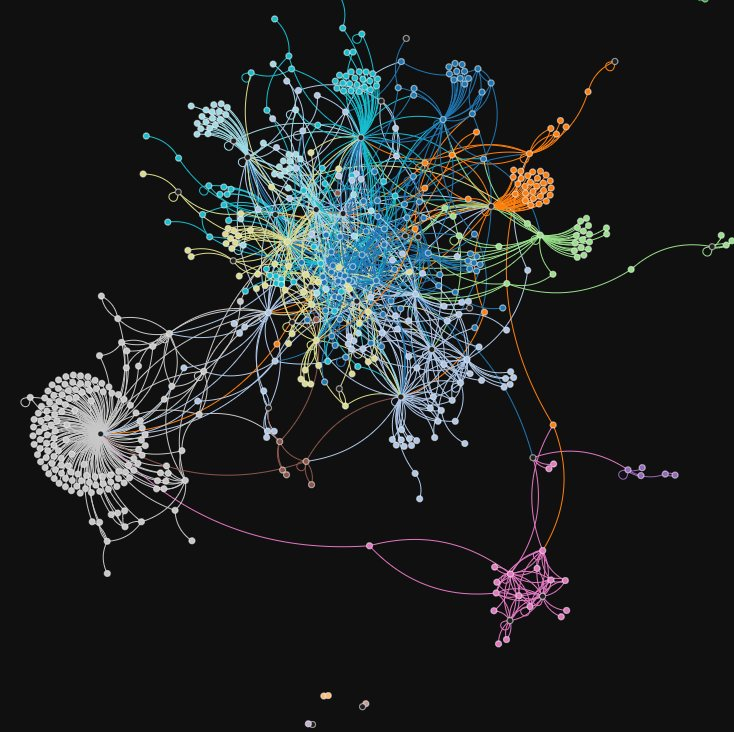
\includegraphics[width=.6\linewidth]{./Pictures/innovatoripa_01.jpg}\label{fig:InnoNet}
	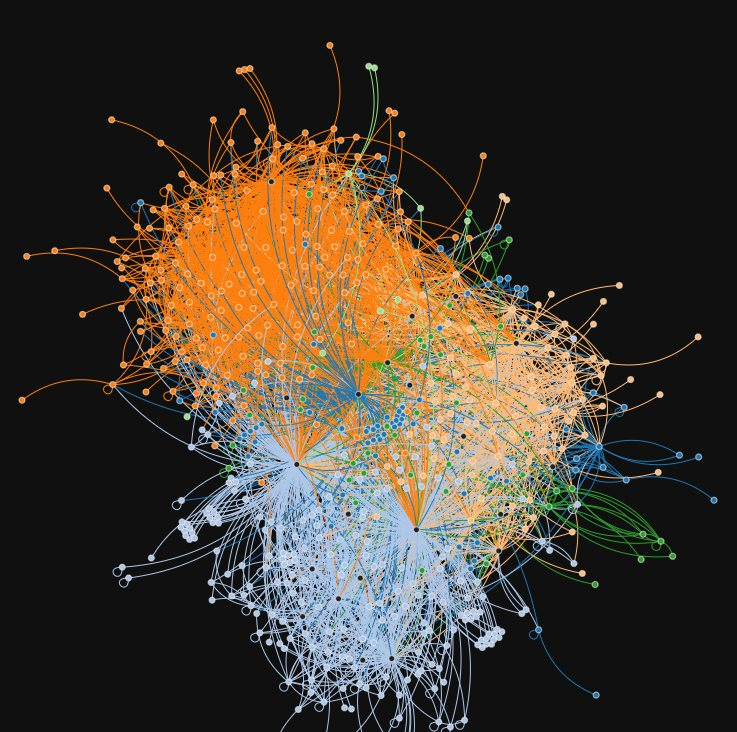
\includegraphics[width=.6\linewidth]{./Pictures/edgeryders_02.jpg}\label{fig:EdgeNet}
  	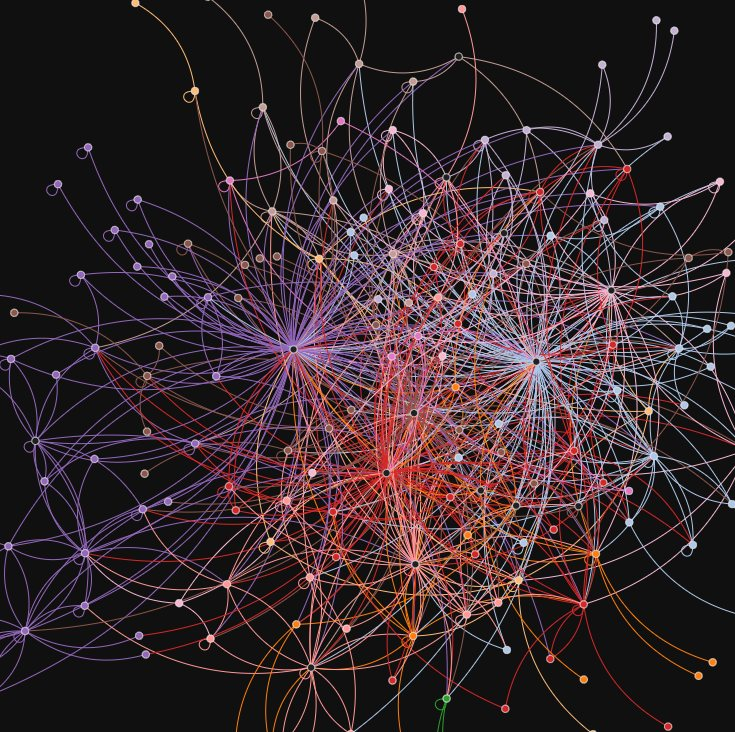
\includegraphics[width=.6\linewidth]{./Pictures/matera2019_01.jpg}\label{fig:MT2019Net}
  %\subfloat[][]{}
    %\subfloat[][]{}
  \caption{Interaction networks of three small online communities. Innovatori PA (top) does not have an onboarding policy in place, whereas the two others do.} 
 \label{fig:NetViz}
\end{figure}

We fit power laws in-degree distributions of these three online communities, as of early December 2014. Next, we tested the hypothesis that degree distributions follow a power law, as predicted by the theory. This was done in the following way:
\begin{enumerate}
\item first, we fitted power functions to the entire support of each in-degree distribution, i.e. for any degree greater than or equal to 1. 
\item next, we fitted power functions to the right tail of each in-degree distribution, i.e. for any degree greater than or equal to $k_{min}$, where $k_{min}$ is the in-degree that minimizes the Kolmogorov-Smirnov distance between the fitted function and the data with in-degree $k \geq k_{min}$.
\item finally, we ran goodness-of-fit tests for each in-degree distribution and for fitted power functions as described in both 1 and 2. The null hypothesis tested is that the observed distribution is generated by a power function with exponent $\alpha$. We used a test based on comparing the Kolmogorov-Smirnov $D$ statistic of the observed distribution with those of a large number of synthetic datasets drawn by the fitted power function. Such comparison is summarized in a p-value, that indicates the probability of the $D$ statistic to exceed the observed value conditional to the null hypothesis being true. Observing p-values close to 1 indicate that the power function is a good fit for the data, and do not allow rejection of the null hypothesis; p-values close to zero indicate that the power function is a bad fit for the data, and lead to reject the null hypothesis. The rejection value is set, conservatively, at 0.1.  The method we followed is borrowed from Clauset, Shalizi and Newman \cite{clauset2009power} and is described in detail in the Appendix. 
\end{enumerate}
	
\begin{figure*}
\centering
	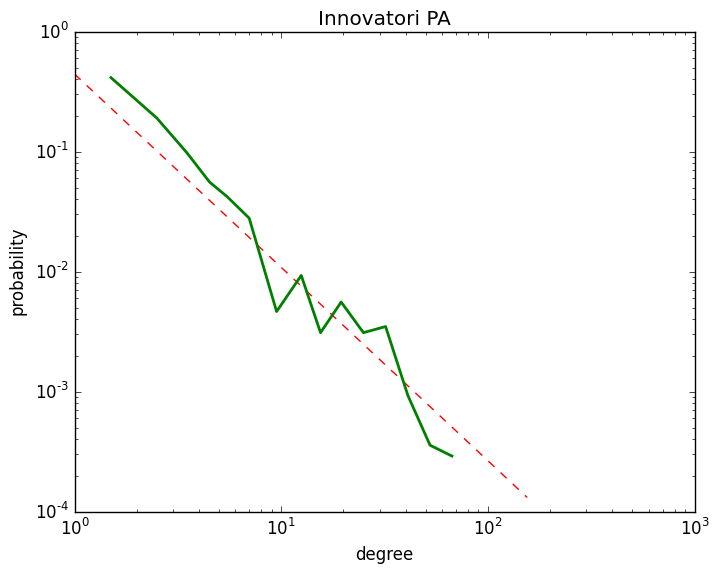
\includegraphics[width=.45\linewidth]{./Pictures/PDF_fit_innovatoriPA.png}\label{fig:fit_innovatoriPA}
	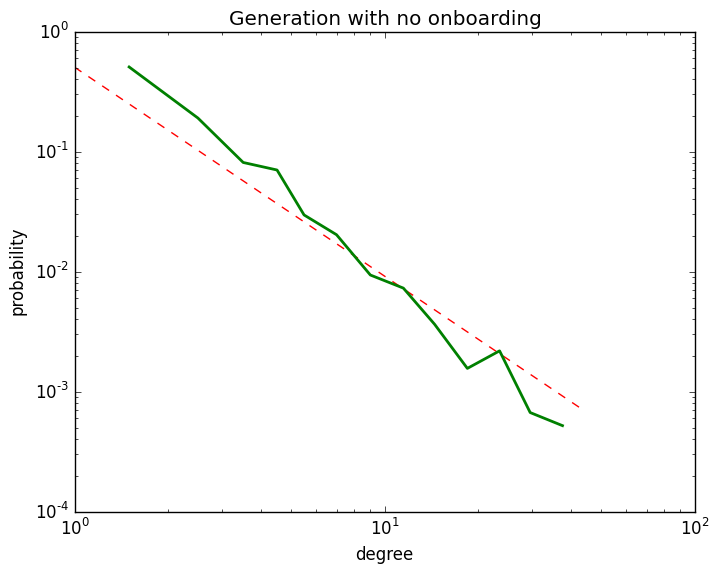
\includegraphics[width=.45\linewidth]{./Pictures/YES_PDF_fit_no_onboarding_178.png}\label{fig:fit_no_onboarding}
	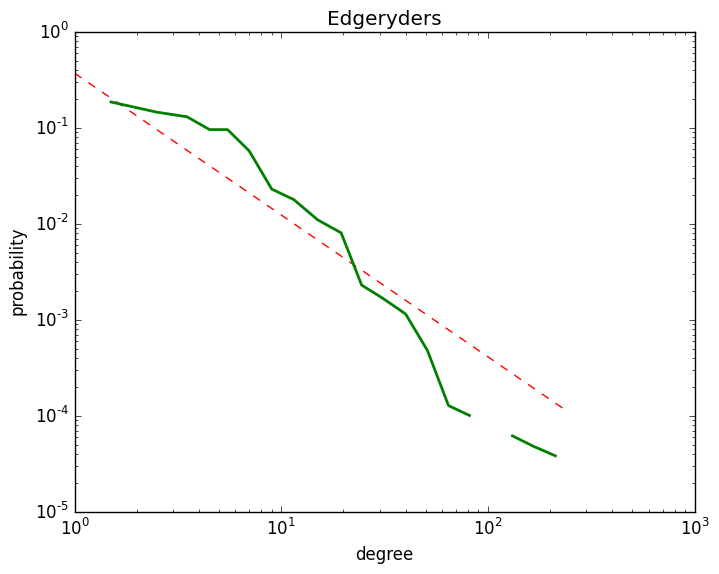
\includegraphics[width=.45\linewidth]{./Pictures/PDF_fit_edgeryders.png}\label{fig:fit_edgeryders}
	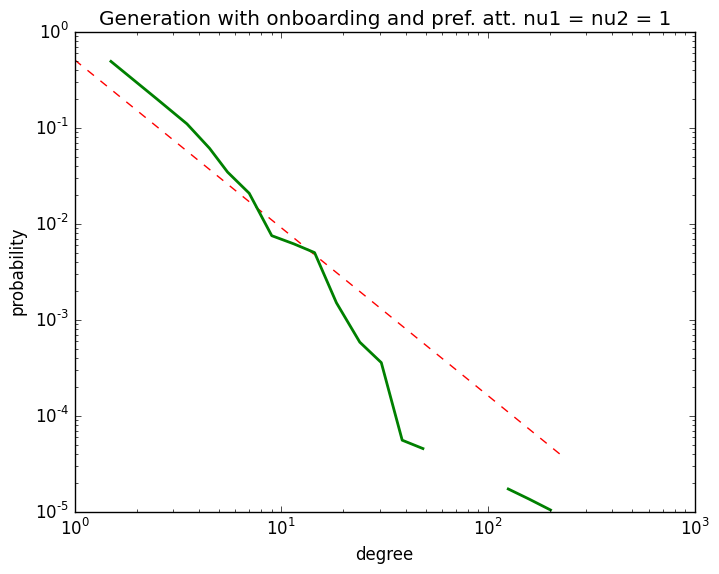
\includegraphics[width=.45\linewidth]{./Pictures/YES-PDF_fit_onboarding_nu_1_1__429.png}\label{fig:fit_nu_1_1}
  %\subfloat[][]{}
  %\subfloat[][]{}
  \caption{Probability density function from the degree distributions of: (Top) the Innovatori PA network without \emph{onboarding} policy in place versus a generated model without \emph{onboarding} either.
  (Bottom) The Edgeryders network with \emph{onboarding} and preferential attachment vers a generated model with onboarding and maximal preferential attachments ($\nu_1 = \nu_2 = 1$).}
 \label{fig:PDFViz}
\end{figure*}

We emphasize in-degree, as opposed to out-degree, for the following reason. The Barab\'asi-Albert model and many of its extensions \cite{dorogovtsev2002evolution} have been applied to undirected as well as to directed network. However, directedness is implicit in the idea of preferential attachment; new nodes "choose" who to link to. When networks are directed, it is reasonable to expect the in-degree distribution to be the one to follow a power law. This expectation has been confirmed by empirical investigation \cite{dorogovtsev2002evolution}, supporting the conjecture that some preferential attachment is present in many in online conversation networks. As new members join, many of them will reach out to someone, and it seems to make sense that they will target highly connected individuals more. 

Results are summarised in Table \ref{table:goodnessOfFit}. 

\begin{table}[b]
\centering 
\begin{tabular}{| c | c | c | c |} 
\hline 
& \quad exponent \quad  & \quad $k_{min}$ \quad & \quad $p$-value \quad \\ 
\hline 
%Innovatori PA  $k \geq 1$ & 1.611 & 1 & 0.21 \\
%\hline 
%Innovatori PA $k \geq k_{min}$  & 1.834 & 2 & 0.76 \\
%\hline
%Edgeryders $k \geq 1$ & 1.477 & 1 & 0.00 - \emph{reject} \\
%\hline
%Edgeryders $k \geq k_{min}$ & 2.250 & 5 & 0.45 \\
%\hline
%Matera2019 $k \geq 1$ & 1.506 & 1 & 0.00 - \emph{reject} \\
%\hline
%Matera2019 $k \geq k_{min}$ & 2.817 & 6 & 0.94 \\
\quad Innovatori PA  $k \geq 1$ \quad & \quad 1.611 \quad & \quad 1 \quad & \quad 0.21 \quad \\
\hline 
\quad Innovatori PA $k \geq k_{min}$  \quad & \quad 1.834 \quad & \quad 2 \quad & \quad 0.76 \quad \\
\hline
\quad Edgeryders $k \geq 1$ \quad & \quad 1.477 \quad & \quad 1 \quad & \quad 0.00 - \emph{reject} \quad \\
\hline
\quad Edgeryders $k \geq k_{min}$ \quad & \quad 2.250 \quad & \quad 5 \quad & \quad 0.45 \quad \\
\hline
\quad Matera2019 $k \geq 1$ \quad & \quad 1.506 \quad & \quad 1 \quad & \quad 0.00 - \emph{reject} \quad \\
\hline
\quad Matera2019 $k \geq k_{min}$ \quad & \quad 2.817 \quad & \quad 6 \quad & \quad 0.94 \quad \\
\hline 
\end{tabular}
\caption{Testing for goodness-of-fit of power functions to interaction networks of degree distributions in three online communities.}
\label{table:goodnessOfFit}
\end{table}

As we consider the interval  $k \geq 1$, we find that the in-degree distribution of the Innovatori PA interaction network, the unmoderated one, is consistent with the expected behaviour of an evolving network with preferential attachment; we cannot reject the null hypothesis that it was generated by a power law. The same is not true of the other two online communities, both with onboarding policies, for which the null hypothesis is strongly rejected.  

When we consider only the tail of the degree distributions, i.e. degree distributions for $k \geq k_{min}$, on the other hand, all three communities display a behaviour that is consistent with that of evolving networks with preferential attachment.

This set of results is consistent with the objectives of the onboarding policy. These consist of helping newcomers to overcome the initial difficulties associated with finding your way around an online community that they don't know yet. A successfully onboarded new user will generally have some extra interaction with existing community members with respect to ones that are left to themselves; all things being equal, we can expect this to lead to extra edges appearing in the interaction network, and interfering with the in-degree distribution that would appear in the absence of onboarding. This could explain the non-power law in-degree distribution of Edgeryders and Matera2019. On the other hand, it is reasonable to expect this interference to concern mostly low connectivity nodes: onboarding targets predominantly newcomers, and focuses on helping them through the first few successful interactions. Highly active (therefore highly connected) community members do not need to be onboarded. This could explain why, when we consider only the highly connected nodes in the distribution's upper tails, all three communities display similar behaviour, regardless of onboarding policies. 

\subsection{Experiment protocol}
The difference observed between the two communities with onboarding policies and the one without might be caused not by the policy itself, but by some other unobserved variable. To explore the issue further, we generate and compare computer simulations of interaction networks in online communities that are identical except for the presence and effectiveness of onboarding policies. Communities are assumed to grow over time, with new participants joining them in sequence; at each point in time, new edges appear; their probability of targeting an existing node grows linearly with that node's in-degree. Additionally, communities might have or not have onboarding policies. For those communities that do have them, they are modelled by means of two scalar parameters $\nu_1$  and $\nu_2$ , that vary between 0 and 1. The first one captures onboarding effectiveness;  the second one captures community responsiveness. As they get closer to 1, the community manager's onboarding action gets closer to having the desired effects. In the next subsection, we specify the model and define more specifically the meaning of both parameters.

We proceed as follows.

First, we simulate the evolution of the interaction network of a large number of online communities. Divide them into a control group (no onboarding policy) and a treatment group (presence of onboarding policy). Specifically, we simulate the evolution of the interaction network of:

\begin{itemize}
\item 100 communities with no onboarding policy. These will constitute the control group of our simulated communities. 
\item 100 communities for each couple of values of $\nu_1$  and $\nu_2$, with $\nu_1, \nu_2 \in \{0.0, 0.2, 0.4, 0.6, 0.8, 1.0\}$. These will constitute our treatment groups.
\item For each of these networks, we compute the in-degree distribution.
\end{itemize}

Next, we define the following hypotheses. 

\begin{itemize}
\item Let $C$ be the network of interaction in an online community. Denote the in-degree of nodes in the network by $k$. Let $P$ be the best-fit power-law model for the in-degree distribution of $C$.
\item \emph{Hypothesis 1}. The in-degree distribution of $C$ is generated by $P$ for any $k \geq 1$.
\item \emph{Hypothesis 2}. The in-degree distribution of $C$ is generated by $P$ for any $k \geq k_{min}$, where $k_{min}$ is the in-degree that minimizes the Kolmogorov-Smirnov distance between the fitted function and the data over $k \geq k_{min}$.
\end{itemize}

Finally, we test Hypothesis 1 and 2 on each of the 3700 in-degree distributions generated. We do this using the goodness-of-fit tests proposed by Clauset et.al. \cite{clauset2009power} and illustrated in detail in the Appendix. We expect to obtain the following:

\begin{itemize}
\item In the control group, both Hypothesis 1 and Hypothesis 2 are true. 
\item In the treatment group with fully effective onboarding Hypothesis 1 is false and Hypothesis 2 is true. 
\item In the intermediate situations of partially ineffective onboarding, Hypothesis 1 can be true or false, according to the value of $\nu_1$ and $\nu_2$. Hypothesis 2 is true.
\end{itemize}


\subsection{The simulation model}

Our computer model simulates the growth of an interaction network in an online community with and without onboarding.  

\subsubsection*{Without onboarding}

We use the model without onboarding to generate the networks in our control group. Its growth mechanism for the network to grow is based on preferential attachment, consistently with the Barab·si-Albert tradition. We follow the more general formulation of Dorogovtsev and Mendes \cite{dorogovtsev2002evolution}.
\begin{itemize}
\item A network is initialized, consisting of two reciprocally connected nodes
\item At each time step, one new node -- representing a participant in the online community -- appears in the network. 
\item At each time step, $m$ new edges --  representing comments --  appear in the network. The source of each edge is drawn at random from the uniform distribution of the existing nodes\footnote{This represents a departure from \cite{dorogovtsev2002evolution}, where edge sources are assumed to be unspecified. We need to specify edge sources in order to conform to the data model of the network analysis softwares we are using; this, however, does not have any analytical implications, as both \cite{dorogovtsev2002evolution} and we focus on the in-degree distribution.}. Its target is chosen according to the following rule: the probability that the new edge points to node $s$ is proportional to $k(s) + A_s$ where $A_s$ is a parameter representing additional attractiveness of the node.
\end{itemize}

\subsubsection*{With onboarding}

We use a variant of the above model that includes onboarding to generate the networks in our treatment group. The variant consists simply of the model without onboarding, to which further steps are added as follows.
\begin{itemize}
\item At each timestep, one edge is directed towards the newcomer node. This is meant to represent the community manager's onboarding action described in section 1. 
\item At each timestep, with probability $\nu_1$, one edge is added. Its source is the newcomer node; its target is chosen according to the following rule: the probability that the new edge points to node $s$ is proportional to $k(s) + A$ where $A$ is a parameter representing additional attractiveness of the node. This is meant to represent the newcomer's reaction to the community manager's onboarding activity; as a result of the latter, the newcomer becomes active and reaches out to someone in the community, as advised by the community manager. We assume that community managers will normally incline to point newcomers to existing users who are reputed to be interesting conversationalists, and that the characteristic of being interesting conversationalists is correlated with node in-degree. Parameter $\nu_1$ can be thought of as representing \emph{onboarding effectiveness}. More skilled community managers will be more persuasive in inducing newcomers to reach out and engage in the conversation taking place in the online community.
\item At each timestep, with probability $\nu_2$, one edge is added. Its source is drawn at random from the uniform distribution of the existing nodes; its target is the newcomer node. This represents a successful onboarding outcome: the new participant, by becoming active, has attracted the attention of some existing participant, who has engaged with her. The new participant, no longer isolated, is now in conversation. $\nu_2$ can be thought of as representing \emph{community responsiveness}. As it increases, the efforts of newcomers to engage in conversation become more likely to be reciprocated.
\end{itemize}


\section{Results} \label{sec:results}
Following the protocol outlined above, we evolved 100 networks for each of the 37 variants of the model. For all networks, we set network size to 2000 nodes; $A = 1$; and $m = 1$. These choices are discussed in the appendix.

\subsection{Goodness-of-fit of the power-law model} \label{ssec:GOF of power law}

For each network evolved we computed two best-fit power-law models, one for $k \geq 1$ and the other for $k\geq k_{min}$ where $k_{min}$ is the in-degree the minimizes the Kolmogorov-Smirnov distance between the fitted function and the data over $k \geq k_{min}$. On each of these models, we ran a goodness-of-fit test as described in section 3.2. This resulted in two distributions of p-values for our control group, plus two more for each of our six treatment groups. Table \ref{table:GOF1}
 and \ref{table:AvgPvall} report descriptive statistics for these distributions.

\begin{table}[h]
\centering
\caption{Number of rejects (out of 100 runs) for goodness-of-fit tests of power-law models to in-degree distributions of interaction networks in online communities, with no onboarding (control group) and with onboarding. Power-law models are estimated over all nodes with degree $k \geq 1$}
\label{table:GOF1}
\begin{tabular}{lcccccc}
\hline
\multicolumn{7}{c} {Control group: 23}\\
\hline
%& $\nu_2$ = 0.0 & $\nu_2$ = 0.2 & $\nu_2$ = 0.4 & $\nu_2$ = 0.6 & $\nu_2$ = 0.8 & $\nu_2$ = 1\\
%$\nu_1$ = 0.0          & 83        & 81        & 83        & 88        & 82        & 85      \\
%$\nu_1$ = 0.2          & 78        & 73        & 70        & 73        & 73        & 70      \\
%$\nu_1$ = 0.4          & 66        & 65        & 61        & 69        & 76        & 56      \\
%$\nu_1$ = 0.6          & 59        & 67        & 63        & 51        & 70        & 71      \\
%$\nu_1$ = 0.8          & 55        & 60        & 66        & 61        & 60        & 61      \\
%$\nu_1$ = 1            & 65        & 62        & 54        & 60        & 54        & 57   \\
\quad & \quad $\nu_2$ = 0.0 \quad & \quad $\nu_2$ = 0.2 \quad & \quad $\nu_2$ = 0.4 \quad & \quad $\nu_2$ = 0.6 \quad & \quad $\nu_2$ = 0.8 \quad & \quad $\nu_2$ = 1\quad \\
\quad $\nu_1$ = 0.0          \quad & \quad 83        \quad & \quad 81        \quad & \quad 83        \quad & \quad 88        \quad & \quad 82        \quad & \quad 85      \quad \\
\quad $\nu_1$ = 0.2          \quad & \quad 78        \quad & \quad 73        \quad & \quad 70        \quad & \quad 73        \quad & \quad 73        \quad & \quad 70      \quad \\
\quad $\nu_1$ = 0.4          \quad & \quad 66        \quad & \quad 65        \quad & \quad 61        \quad & \quad 69        \quad & \quad 76        \quad & \quad 56      \quad \\
\quad $\nu_1$ = 0.6          \quad & \quad 59        \quad & \quad 67        \quad & \quad 63        \quad & \quad 51        \quad & \quad 70        \quad & \quad 71      \quad \\
\quad $\nu_1$ = 0.8          \quad & \quad 55        \quad & \quad 60        \quad & \quad 66        \quad & \quad 61        \quad & \quad 60        \quad & \quad 61      \quad \\
\quad $\nu_1$ = 1            \quad & \quad 65        \quad & \quad 62        \quad & \quad 54        \quad & \quad 60        \quad & \quad 54        \quad & \quad 57   \quad \\
\hline  
\end{tabular}
\end{table}


Table \ref{table:GOF1} shows a count of the networks for which the goodness-of-fit test returns a p-value below 0.1 (the threshold value below which the literature recommend Hypothesis 1 is rejected), out of the 100 runs. From it, we conclude that onboarding seems to have some effect on the goodness-of-fit of the generated data to their respective best-fit power-law models when $k \geq 1$. The effect goes in the direction of reducing the p-values.

It is worth to look at the average p-values generated by each combination of $\nu_1$ and $\nu_2$. These are shown in Table \ref{table:AvgPvall}.

\begin{table}[h]
\centering
\caption{Average p-values for goodness-of-fit tests of power-law models to in-degree distributions of interaction networks in online communities, with no onboarding (control group) and with onboarding. Power-law models are estimated over all nodes with degree $k \geq 1$}
\label{table:AvgPvall}
\begin{tabular}{lllllll}
\hline
\multicolumn{7}{c} {Control group: 0.262688}\\
\hline
%Average p-value & $\nu_2$ = 0.0 & $\nu_2$ = 0.2 & $\nu_2$ = 0.4 & $\nu_2$ = 0.6 & $\nu_2$ = 0.8 & $\nu_2$ = 1  \\
%$\nu_1$ = 0.0       & 0.059312  & 0.060096  & 0.05196   & 0.047936  & 0.055072  & 0.051396 \\
%$\nu_1$ = 0.2       & 0.062904  & 0.079656  & 0.085248  & 0.083412  & 0.083412  & 0.079596 \\
%$\nu_1$ = 0,4       & 0.104688  & 0.097     & 0.098604  & 0.083072  & 0.082916  & 0.11566  \\
%$\nu_1$ = 0.6       & 0.0964    & 0.085496  & 0.10212   & 0.126872  & 0.090588  & 0.079652 \\
%$\nu_1$ = 0.8       & 0.132616  & 0.115176  & 0.103616  & 0.109108  & 0.118828  & 0.122788 \\
%$\nu_1$ = 1         & 0.100868  & 0.120676  & 0.132564  & 0.116448  & 0.123024  & 0.120464\\
Average p-value \quad & \quad $\nu_2$ = 0.0 \quad & \quad $\nu_2$ = 0.2 \quad & \quad $\nu_2$ = 0.4 \quad & \quad $\nu_2$ = 0.6 \quad & \quad $\nu_2$ = 0.8 \quad & \quad $\nu_2$ = 1  \quad \\
\quad $\nu_1$ = 0.0       \quad & \quad 0.059312  \quad & \quad 0.060096  \quad & \quad 0.05196   \quad & \quad 0.047936  \quad & \quad 0.055072  \quad & \quad 0.051396 \quad \\
\quad $\nu_1$ = 0.2       \quad & \quad 0.062904  \quad & \quad 0.079656  \quad & \quad 0.085248  \quad & \quad 0.083412  \quad & \quad 0.083412  \quad & \quad 0.079596 \quad \\
\quad $\nu_1$ = 0,4       \quad & \quad 0.104688  \quad & \quad 0.097     \quad & \quad 0.098604  \quad & \quad 0.083072  \quad & \quad 0.082916  \quad & \quad 0.11566  \quad \\
\quad $\nu_1$ = 0.6       \quad & \quad 0.0964    \quad & \quad 0.085496  \quad & \quad 0.10212   \quad & \quad 0.126872  \quad & \quad 0.090588  \quad & \quad 0.079652 \quad \\
\quad $\nu_1$ = 0.8       \quad & \quad 0.132616  \quad & \quad 0.115176  \quad & \quad 0.103616  \quad & \quad 0.109108  \quad & \quad 0.118828  \quad & \quad 0.122788 \quad \\
\quad $\nu_1$ = 1         \quad & \quad 0.100868  \quad & \quad 0.120676  \quad & \quad 0.132564  \quad & \quad 0.116448  \quad & \quad 0.123024  \quad & \quad 0.120464\quad \\
\hline
\end{tabular}
\end{table} 

Running t-tests of the null hypothesis that the average p-value in the control group is equal to the average p-values in the different treatment groups results in a strong rejection of the null for any combination of $\nu_1$ and $\nu_2$. It seems unquestionable that introducing onboarding to an online community has a measurable negative impact on the probability of a power-law model to be a good fit for its interaction network's in-degree distribution.

We now turn to the question of the role played by $\nu_1$ and $\nu_2$ within the treatment group. Figure \ref{fig:CDFpvanu_1nu_2} show the cumulate density functions of the p-values in the control and treatment groups as $\nu_1$ and $\nu_2$ vary. 

\begin{figure}[thb]
\centering

	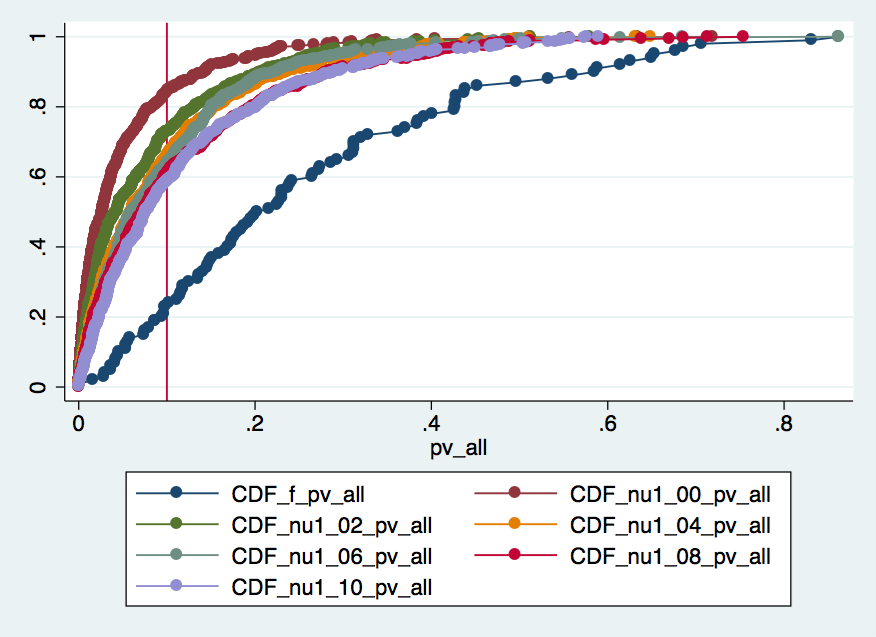
\includegraphics[width=.75\linewidth]{./Pictures/CDF_pva_nu1.png}\label{fig:CDFnu_1}
	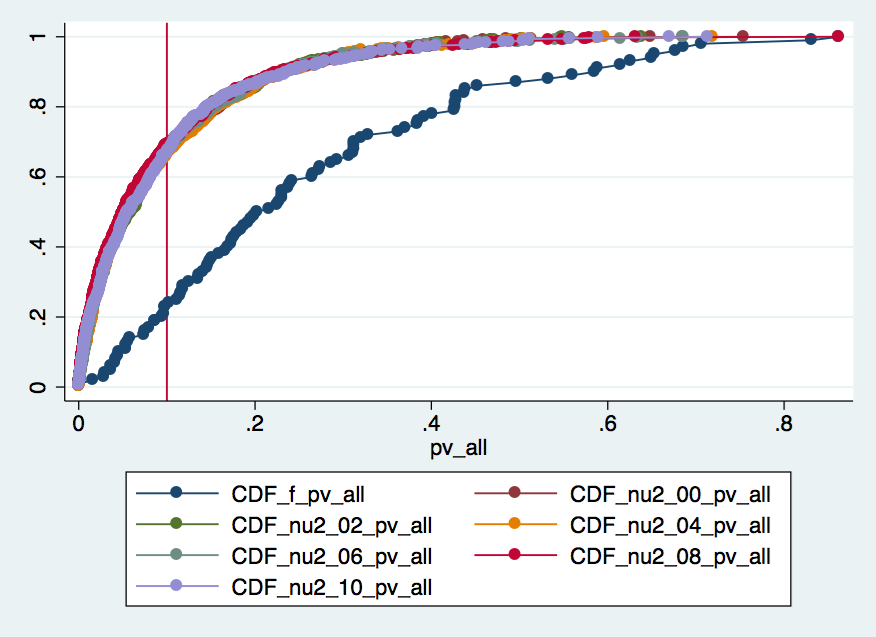
\includegraphics[width=.75\linewidth]{./Pictures/CDF_pva_nu2.png}\label{fig:CDFnu_2}
  %\subfloat[][]{}
  %\subfloat[][]{}
  \caption{Cumulate Density Functions of p-values returned by goodness-of-fit tests to the (best-fit) power-law models for in-degree distributions of the interaction networks in the control and treatment groups. 20\% of the networks evolved without onboarding (dark blue) have degree distributions that test negatively for H1. When onboarding is introduced, that percentage rises to between 50 and 90\%. Above, the treatment group interaction networks have been grouped according to the value taken by $\nu_1$; below, they have been grouped according to the value taken by $\nu_2$ } 
 \label{fig:CDFpvanu_1nu_2}
\end{figure}

Onboarding effectiveness $\nu_1$ and community responsiveness $\nu_2$ seem to affect the in-degree distributions in different ways. Increasing $\nu_1$ pushes average p-values of the goodness-of-fit tests down, making it less likely that Hypothesis 1 would be rejected. Increasing $\nu_2$ seems not to play any role at all. This is somewhat surprising; higher values of $\nu_2$ lead to allocating an extra edge to the newcomer, and we have seen that allocating the first one (which is what happens when onboarding is introduced) has a strong negative effect on the p-value returned by the goodness-of-fit test. 

Regression analysis confirms the intuition from Figure \ref{fig:CDFpvanu_1nu_2}. We generated 6 dummy variables, each taking value 1 when $\nu_1 =  c$ and 0 otherwise, with $c \in \{0.0, 0.2, 0.4, 0.6, 0.8, 1\}$; next we generated 6 more dummy variables for the same vaules of $\nu_2$ . We then estimated a linear regression model with the p-value of our goodness-of-fit test as the dependent variable and the 12 dummy variables as its predictors. The results are:

\begin{enumerate}
\item Coefficients on predictors corresponding to different values of $\nu_1$ are positive and significant at the 0.05 level or better, with the exception of that corresponding to $\nu_1 = 0.2$.
\item Coefficients on predictors corresponding to different values of $\nu_2$ are non-significant.
\item Coefficients on interaction terms between $\nu_1$ and $\nu_2$ are non-significant.
\item A F-test of joint significance of the group of predictors corresponding to different values of $\nu_1$ strongly rejects the null hypothesis of non-significance (p-value: 0.0000).
\item A F-test of joint significance of the group of predictors corresponding to different values of $\nu_2$ does not reject the null hypothesis of non-significance (p-value: 0.9623).
\item A F-test of joint significance of the interaction terms does not reject the null hypothesis of non-significance (p-value: 0.1553).
\end{enumerate}

Full regression results are available in the appendix.

When we consider only the upper tail of the in-degree distribution ($k \geq 1$), the effect of introducing onboarding on the goodness-of-fit is much less clear. All but 32 (out of 3600) networks in the treatment group give rise to in-degree distributions that turn out to be a good fit for a power-law model when $k_{min}$ is chosen so as to minimize the Kolmogorov-Smirnov distance between the degree distributions themselves and their best-fit power-law models. We conclude that we do not reject Hypothesis 2, regardless of whether onboarding is present or not. This is illustrated by Table \ref{table:rejectsNoOb}

\begin{table}[h]
\centering
\caption{Number of rejects (out of 100 runs) for goodness-of-fit tests of power-law models to in-degree distributions of interaction networks in online communities, with no onboarding (control group) and with onboarding. Power-law models are estimated over all nodes with degree $k \geq k_{min}$}
\label{table:rejectsNoOb}
\begin{tabular}{lllllll}
\hline
\multicolumn{7}{c} {Control group: 0}\\
\hline
%  & $\nu_2$ = 0.0 & $\nu_2$ = 0.2 & $\nu_2$ = 0.4 & $\nu_2$ = 0.6 & $\nu_2$ = 0.8 & $\nu_2$ = 1\\
%$\nu_1$ = 0.0        & 1        & 1        & 0        & 0        & 3        & 1      \\
%$\nu_1$ = 0.2          & 1        & 0        & 1        & 3        & 1        & 1      \\
%$\nu_1$ = 0.4          & 1        & 1        & 0        & 2        & 2        & 0      \\
%$\nu_1$ = 0.6          & 0        & 0        & 2        & 1        & 1        & 0      \\
%$\nu_1$ = 0.8          & 1        & 1        & 1        & 3        & 1        & 1      \\
%$\nu_1$ = 1            & 0        & 0        & 1        & 0        & 0        & 0   \\
  \quad & \quad $\nu_2$ = 0.0 \quad & \quad $\nu_2$ = 0.2 \quad & \quad $\nu_2$ = 0.4 \quad & \quad $\nu_2$ = 0.6 \quad & \quad $\nu_2$ = 0.8 \quad & \quad $\nu_2$ = 1\quad \\
\quad $\nu_1$ = 0.0        \quad & \quad 1        \quad & \quad 1        \quad & \quad 0        \quad & \quad 0        \quad & \quad 3        \quad & \quad 1      \quad \\
\quad $\nu_1$ = 0.2          \quad & \quad 1        \quad & \quad 0        \quad & \quad 1        \quad & \quad 3        \quad & \quad 1        \quad & \quad 1      \quad \\
\quad $\nu_1$ = 0.4          \quad & \quad 1        \quad & \quad 1        \quad & \quad 0        \quad & \quad 2        \quad & \quad 2        \quad & \quad 0      \quad \\
\quad $\nu_1$ = 0.6          \quad & \quad 0        \quad & \quad 0        \quad & \quad 2        \quad & \quad 1        \quad & \quad 1        \quad & \quad 0      \quad \\
\quad $\nu_1$ = 0.8          \quad & \quad 1        \quad & \quad 1        \quad & \quad 1        \quad & \quad 3        \quad & \quad 1        \quad & \quad 1      \quad \\
\quad $\nu_1$ = 1            \quad & \quad 0        \quad & \quad 0        \quad & \quad 1        \quad & \quad 0        \quad & \quad 0        \quad & \quad 0   \quad \\
\hline  
\end{tabular}
\end{table}


\subsection{Lower bounds} \label {ssec:lower bounds}

Our results show a limited, albeit statistically significant, effect of onboarding on the value of $k_{min}$, the value of $k$ that minimizes the Kolmogorov-Smirnov distance between the data generated by the computer simulation and the best-fit power-law model. Table \ref {table:ttestkMin} illustrates, for each value of  $\nu_1$ and $\nu_2$, the average value of $k_{min}$, and the result (expressed in p-value) of a t-test on the null hypothesis that such average value is the same as the corresponding statistics in the control group, against the alternative hypothesis that the former is greater than the latter. 

\begin{table}[h]
\centering
\caption{Average values of $k_{min}$ in the control group and in the treatment group by values of $\nu_1$ and $\nu_2$. The number in parenthesis is the p-value associated to a t-test that  $k_{min}(treatment) = k_{min}(control)$. }
\label{table:ttestkMin}
\begin{tabular}{lllllll}
\hline
\multicolumn{7}{c} {Control group: 3.43}\\
\hline
%  & $\nu_2$ = 0.0 & $\nu_2$ = 0.2 & $\nu_2$ = 0.4 & $\nu_2$ = 0.6 & $\nu_2$ = 0.8 & $\nu_2$ = 1\\
%$\nu_1$ = 0.0        & 3.88 (0.003)        & 3.91 (0.002)         & 3.87 (0.003)        & 3.74 (0.035)        & 3.87 (0.001)        & 3.98 (0.000)      \\
%$\nu_1$ = 0.2          & 3.95 (0.000)        & 3.92 (0.001)        & 4.06 (0.000)        & 3.94 (0.001)        & 3.84 (0.004)        & 3.99 (0.001)      \\
%$\nu_1$ = 0.4          & 4.2 (0.000)        & 4.11 (0.000)        & 4.14 (0.000)        & 3.91 (0.001)        & 4.04 (0.000)        & 4.21 (0.000)      \\
%$\nu_1$ = 0.6          & 4.31 (0.000)        & 4.17 (0.000)        & 4.14 (0.000)        & 4.22 (0.000)        & 4.2 (0.000)        & 3.96 (0.000)      \\
%$\nu_1$ = 0.8          & 4.23 (0.000)        & 4.55 (0.000)        & 4.22 (0.000)        & 4.14 (0.000)        & 4.17 (0.000)        & 4.27 (0.000)      \\
%$\nu_1$ = 1            & 4.16 (0.000)         & 4.58 (0.000)        & 4.49 (0.000)        & 4.35 (0.000)        & 4.39 (0.000)        & 4.24 (0.000)   \\
  \quad & \quad $\nu_2$ = 0.0 \quad & \quad $\nu_2$ = 0.2 \quad & \quad $\nu_2$ = 0.4 \quad & \quad $\nu_2$ = 0.6 \quad & \quad $\nu_2$ = 0.8 \quad & \quad $\nu_2$ = 1\quad \\
\quad $\nu_1$ = 0.0        \quad & \quad 3.88 (0.003)        \quad & \quad 3.91 (0.002)         \quad & \quad 3.87 (0.003)        \quad & \quad 3.74 (0.035)        \quad & \quad 3.87 (0.001)        \quad & \quad 3.98 (0.000)      \quad \\
\quad $\nu_1$ = 0.2          \quad & \quad 3.95 (0.000)        \quad & \quad 3.92 (0.001)        \quad & \quad 4.06 (0.000)        \quad & \quad 3.94 (0.001)        \quad & \quad 3.84 (0.004)        \quad & \quad 3.99 (0.001)      \quad \\
\quad $\nu_1$ = 0.4          \quad & \quad 4.2 (0.000)        \quad & \quad 4.11 (0.000)        \quad & \quad 4.14 (0.000)        \quad & \quad 3.91 (0.001)        \quad & \quad 4.04 (0.000)        \quad & \quad 4.21 (0.000)      \quad \\
\quad $\nu_1$ = 0.6          \quad & \quad 4.31 (0.000)        \quad & \quad 4.17 (0.000)        \quad & \quad 4.14 (0.000)        \quad & \quad 4.22 (0.000)        \quad & \quad 4.2 (0.000)        \quad & \quad 3.96 (0.000)      \quad \\
\quad $\nu_1$ = 0.8          \quad & \quad 4.23 (0.000)        \quad & \quad 4.55 (0.000)        \quad & \quad 4.22 (0.000)        \quad & \quad 4.14 (0.000)        \quad & \quad 4.17 (0.000)        \quad & \quad 4.27 (0.000)      \quad \\
\quad $\nu_1$ = 1            \quad & \quad 4.16 (0.000)         \quad & \quad 4.58 (0.000)        \quad & \quad 4.49 (0.000)        \quad & \quad 4.35 (0.000)        \quad & \quad 4.39 (0.000)        \quad & \quad 4.24 (0.000)   \quad \\
\hline  
\end{tabular}
\end{table}

\begin{figure}[thb]
\centering

	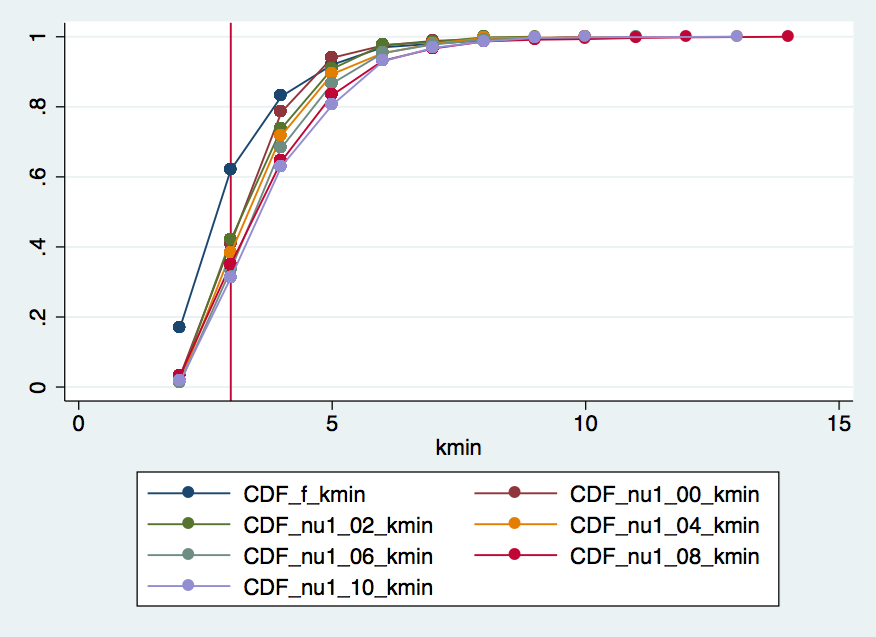
\includegraphics[width=.75\linewidth]{./Pictures/CDF_kmin_nu1.png}
	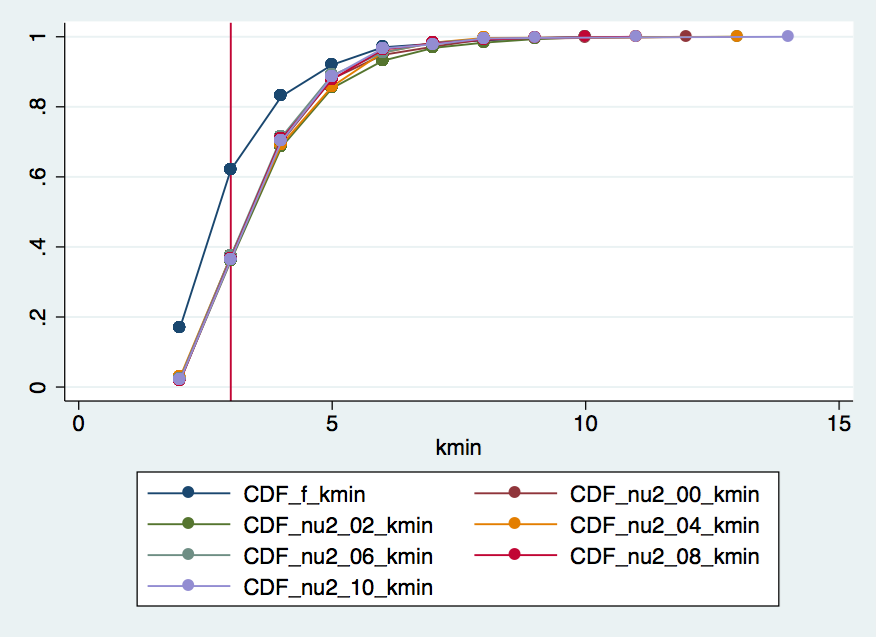
\includegraphics[width=.75\linewidth]{./Pictures/CDF_kmin_nu2.png}
  %\subfloat[][]{}
  %\subfloat[][]{}
  \caption{Cumulate Density Functions of the average value of $k_{min}$ that minimizes the Kolmogorov-Smirnov distance between the in-degree distribution of each interaction network and its best-fit power-law model.  returned by goodness-of-fit tests to the (best-fit) power-law models for in-degree distributions of the interaction networks in the control and treatment groups. 20\% of the networks evolved without onboarding (dark blue) have degree distributions that test negatively for H1. When onboarding is introduced, that percentage rises to between 50 and 90\%. Above, the treatment group interaction networks have been grouped according to the value taken by $\nu_1$; below, they have been grouped according to the value taken by $\nu_2$.} 
 \label{fig:CDFkmin_nu_1nu_2}
\end{figure}



A glance at figure \ref{fig:CDFkmin_nu_1nu_2} shows that over 60\% of the in-degree distributions from interaction networks in the control group, vis-a-vis only 30 to 40\% of those in the treatment group, fit a power-law model best for $k_{min} \leq 3$. Within the treatment group, some variability is associated to the increase of $\nu_1$, whereas $\nu_2$ does not seem to play a significant role. Regression analysis, however, shows that, once we control for the presence of onboarding, neither parameter is significant. To prove this, we proceed analogously to section \ref{ssec:GOF of power law}: we estimated a linear regression model with the value of $k_{min}$ as the dependent variable and the 12 dummy variables as its predictors. The results are:

\begin{enumerate}
\item Coefficients on predictors corresponding to different values of $\nu_1$ are positive but non-significant, with the exception of that corresponding to $\nu_1 = 0.4$.
\item Coefficients on predictors corresponding to different values of $\nu_2$ are non-significant.
\item Coefficients on interaction terms between $\nu_1$ and $\nu_2$ are non-significant.
\item A F-test of joint significance of the group of predictors corresponding to different values of $\nu_1$ does not reject the null hypothesis of non-significance (p-value: 0.1227).
\item A F-test of joint significance of the group of predictors corresponding to different values of $\nu_2$ does not reject the null hypothesis of non-significance (p-value: 0.8682).
\item A F-test of joint significance of the interaction terms does not reject the null hypothesis of non-significance (p-value: 0.7456).
\end{enumerate}

Full regression analysis is available in the appendix.


\subsection{Exponents} \label{ssec:exponents}
We find that introducing onboarding to an online community has a positive and significant on the value of the exponent of the best-fit power-law model for the in-degree distribution of its interaction network. This is consistent with the theoretical results by Dorogovtsev and Mendes \cite{dorogovtsev2002evolution}, who proved that introducing a fraction of non-preferential attachment edges in evolving networks with preferential attachment does not suppress the power-law dependence of its degree distribution, but only increases the scaling exponent thereof. 

This result holds when the best-fit power-law models is computed over $k \geq k_{min}$, where $k_{min}$ is, as usual, the value of $k$ that minimizes the Kolmogorov-Smirnov distance between the simulated in-degree distribution and its best-fit power-law model. When it is computed over the whole support of the in-degree distribution ($k \geq  1$), it also holds, except for $\nu_1 = 1$; in the latter case, the null hypothesis that the values of the exponent in the control and in the treatment groups are drawn from the same distribution cannot be rejected. Tables \ref {table:ttestExpA} and \ref {table:ttestExp} illustrate, for each value of  $\nu_1$ and $|nu_2$, the average value of the scaling parameter $\alpha$, and the result (expressed in p-value) of a t-test on the null hypothesis that such average value is the same as the corresponding statistics in the control group, against the alternative hypothesis that the former is greater than the latter. Table \ref{table:ttestExpA} refers to $k \geq  1$, whereas Table \ref{table:ttestExp} refers to $k_{min}$.

\begin{table}[h]
\centering
\caption{Average values of the power-law model's exponent $\alpha$ in the control group and in the treatment group by values of $\nu_1$ and $\nu_2$, computed over the whole support $k \geq 1$. The number in parenthesis is the p-value associated to a t-test that  $\alpha(treatment) = \alpha(control)$. }
\label{table:ttestExpA}
\begin{tabular}{lllllll}
\hline
\multicolumn{7}{c} {Control group: 1.752}\\
\hline
%  & $\nu_1$ = 0.0 & $\nu_2$ = 0.2 & $\nu_2$ = 0.4 & $\nu_2$ = 0.6 & $\nu_2$ = 0.8 & $\nu_2$ = 1\\
%$\nu_1$ = 0.0        & 1.89 (0.00)        & 1.89 (0.00)         & 1.89 (0.00)        & 1.89 (0.00)        & 1.89 (0.00)        & 1.89 (0.00)      \\
%$\nu_1$ = 0.2          & 1.85 (0.00)        & 1.85 (0.00)        & 1.85 (0.00)        & 1.85 (0.00)        & 1.85 (0.00)        & 1.85 (0.00)      \\
%$\nu_1$ = 0.4          & 1.82 (0.00)        & 1.82 (0.00)        & 1.82 (0.00)        & 1.82 (0.00)        & 1.82 (0.00)        & 1.82 (0.00)      \\
%$\nu_1$ = 0.6          & 1.79 (0.00)        & 1.79 (0.00)        & 1.79 (0.00)        &  1.79 (0.00)        & 1.79 (0.00)        & 1.79 (0.00)      \\
%$\nu_1$ = 0.8          & 1.77 (0.00)        & 1.77 (0.00)        & 1.77 (0.00)        & 1.77 (0.00)        & 1.77 (0.00)        & 1.77 (0.00)      \\
%$\nu_1$ = 1            & 1.75 (0.21)         & 1.75 (0.20)        & 1.75 (0.26)        & 1.75 (0.43)        & 1.75 (0.24)        & 1.75 (0.19)   \\
  \quad & \quad $\nu_1$ = 0.0 \quad & \quad $\nu_2$ = 0.2 \quad & \quad $\nu_2$ = 0.4 \quad & \quad $\nu_2$ = 0.6 \quad & \quad $\nu_2$ = 0.8 \quad & \quad $\nu_2$ = 1\quad \\
\quad $\nu_1$ = 0.0        \quad & \quad 1.89 (0.00)        \quad & \quad 1.89 (0.00)         \quad & \quad 1.89 (0.00)        \quad & \quad 1.89 (0.00)        \quad & \quad 1.89 (0.00)        \quad & \quad 1.89 (0.00)      \quad \\
\quad $\nu_1$ = 0.2          \quad & \quad 1.85 (0.00)        \quad & \quad 1.85 (0.00)        \quad & \quad 1.85 (0.00)        \quad & \quad 1.85 (0.00)        \quad & \quad 1.85 (0.00)        \quad & \quad 1.85 (0.00)      \quad \\
\quad $\nu_1$ = 0.4          \quad & \quad 1.82 (0.00)        \quad & \quad 1.82 (0.00)        \quad & \quad 1.82 (0.00)        \quad & \quad 1.82 (0.00)        \quad & \quad 1.82 (0.00)        \quad & \quad 1.82 (0.00)      \quad \\
\quad $\nu_1$ = 0.6          \quad & \quad 1.79 (0.00)        \quad & \quad 1.79 (0.00)        \quad & \quad 1.79 (0.00)        \quad & \quad  1.79 (0.00)        \quad & \quad 1.79 (0.00)        \quad & \quad 1.79 (0.00)      \quad \\
\quad $\nu_1$ = 0.8          \quad & \quad 1.77 (0.00)        \quad & \quad 1.77 (0.00)        \quad & \quad 1.77 (0.00)        \quad & \quad 1.77 (0.00)        \quad & \quad 1.77 (0.00)        \quad & \quad 1.77 (0.00)      \quad \\
\quad $\nu_1$ = 1            \quad & \quad 1.75 (0.21)         \quad & \quad 1.75 (0.20)        \quad & \quad 1.75 (0.26)        \quad & \quad 1.75 (0.43)        \quad & \quad 1.75 (0.24)        \quad & \quad 1.75 (0.19)   \quad \\
\hline  
\end{tabular}
\end{table}

\begin{table}[h]
\centering
\caption{Average values of the power-law model's exponent $\alpha$ in the control group and in the treatment group by values of $\nu_1$ and $\nu_2$, computed over$k \geq k_{min}$. We omit the p-values associated to a t-test that  $\alpha_{treatment} = \alpha_{control}$, as they are smaller than 0.001 in all cases. }
\label{table:ttestExp}
\begin{tabular}{lllllll}
\hline
\multicolumn{7}{c} {Control group: 2.419}\\
\hline
% & $\nu_2$ = 0.0 & $\nu_2$ = 0.2 & $\nu_2$ = 0.4 & $\nu_2$ = 0.6 & $\nu_2$ = 0.8 & $\nu_2$ = 1\\
%$\nu_1$ = 0.0        & 2.985        & 2.989        & 2.868    & 3.000    & 3.004        & 3.015       \\
%$\nu_1$ = 0.2          & 2.855        & 2.852        & 2.868        & 2.834        & 2.821        & 2.854      \\
%$\nu_1$ = 0.4          & 2.746        & 2.727        & 2.735        & 2.725        & 2.739        & 2.749      \\
%$\nu_1$ = 0.6          & 2.661        & 2.655        & 2.632        & 2.650        & 2.656        & 2.623      \\
%$\nu_1$ = 0.8          & 2.562        & 2.602        & 2.571        & 2.553    & 2.554        & 2.553      \\
%$\nu_1$ = 1            & 2.496        & 2.527        & 2.518        & 2.514        & 2.514        & 2.499   \\
 \quad & \quad $\nu_2$ = 0.0 \quad & \quad $\nu_2$ = 0.2 \quad & \quad $\nu_2$ = 0.4 \quad & \quad $\nu_2$ = 0.6 \quad & \quad $\nu_2$ = 0.8 \quad & \quad $\nu_2$ = 1\quad \\
\quad $\nu_1$ = 0.0        \quad & \quad 2.985        \quad & \quad 2.989        \quad & \quad 2.868    \quad & \quad 3.000    \quad & \quad 3.004        \quad & \quad 3.015       \quad \\
\quad $\nu_1$ = 0.2          \quad & \quad 2.855        \quad & \quad 2.852        \quad & \quad 2.868        \quad & \quad 2.834        \quad & \quad 2.821        \quad & \quad 2.854      \quad \\
\quad $\nu_1$ = 0.4          \quad & \quad 2.746        \quad & \quad 2.727        \quad & \quad 2.735        \quad & \quad 2.725        \quad & \quad 2.739        \quad & \quad 2.749      \quad \\
\quad $\nu_1$ = 0.6          \quad & \quad 2.661        \quad & \quad 2.655        \quad & \quad 2.632        \quad & \quad 2.650        \quad & \quad 2.656        \quad & \quad 2.623      \quad \\
\quad $\nu_1$ = 0.8          \quad & \quad 2.562        \quad & \quad 2.602        \quad & \quad 2.571        \quad & \quad 2.553    \quad & \quad 2.554        \quad & \quad 2.553      \quad \\
\quad $\nu_1$ = 1            \quad & \quad 2.496        \quad & \quad 2.527        \quad & \quad 2.518        \quad & \quad 2.514        \quad & \quad 2.514        \quad & \quad 2.499   \quad \\
\hline  
\end{tabular}
\end{table}

We inspect further the impact of parameters $\nu_1$ and $\nu_2$ via regression analysis. It shows that the former has a significant impact, whereas the latter does not. To prove this, we proceed analogously to section \ref{ssec:GOF of power law}: we estimate two linear regression models with the 12 dummy variables as its predictors. In the first one, the dependent variable is the value of the power-law model's exponent $\alpha$ when the model is estimated over the whole support of the in-degree distribution for each interaction network. In the second one, the dependent variable is power-law model's exponent $\alpha$ when the model is estimated over $k \geq k_{min}$. The results for both models are very similar:

\begin{enumerate}
\item Coefficients on predictors corresponding to different values of $\nu_1$ are negative and highly significant, though small.
\item Coefficients on predictors corresponding to different values of $\nu_2$ are non-significant.
\item Coefficients on interaction terms between $\nu_1$ and $\nu_2$ are non-significant.
\item A F-test of joint significance of the group of predictors corresponding to different values of $\nu_1$ rejects the null hypothesis of non-significance (p-values: 0.000 for both models). 
\item A F-test of joint significance of the group of predictors corresponding to different values of $\nu_2$ does not reject the null hypothesis of non-significance (p-values:  0.4425 for $k  \geq  1$,  0.4034 for $k \geq  k_{min}$).
\item A F-test of joint significance of the interaction terms does not reject the null hypothesis of non-significance (p-values:  0.9177 for $k  \geq  1$,  0.8271 for $k \geq  k_{min}$)  .
\end{enumerate}.

Full regression analysis is available in the appendix.

\section{Discussion}

\subsection{Accounting for degree distribution shape in the interaction networks of online communities}

Our simulation model incorporates two forces. The first one is preferential attachment; the second is onboarding. The former is meant to represent the rich-get-richer effect observed in many real-world social networks; the latter is meant to represent the onboarding action of moderators and community managers. The former's effect is known to lead to the emergence of an in-degree distribution that approximates a power-law model. The latter's effect is more subtle, because it is in turn composed of two effects. The first one consists in the direct action of the moderator, which  always targets the newcomer; the second one by the actions that might be undertaken as a result of well-executed onboarding policy. 

The direct action of the moderators creates edges pointing to nodes not selected by preferential attachment ? this is definitional of onboarding, and of other online community management activities. What (non-moderator) participants in the online community do as a result of moderator activity is not as clear cut. In our simulation model, fully successful onboarding results in extra edges, some of which point to nodes selected by preferential attachment, others to nodes selected otherwise. 

Also, onboarding only targets newcomers in online communities. As many online community management policies, it concerns weakly connected participants in the community: moderators have no need to engage with very active, strongly connected participants, who clearly need no help in getting a conversation going. By doing so, moderators hope to help some shy newcomers turn into active, respected, sought out community members. Once this process is under way, however, moderators have no reason to continue to engage with the same individuals. In terms of our model, this means that newcomers, after having being onboarded, are going to receive new edges by preferential attachment only. It is therefore reasonable to expect that the degree distributions generated by our model display a heavy tail, with the frequency of highly connected nodes following a reasonable approximation of a power law. The overall result of onboarding, then, is an in-degree distribution with power-law behavior for high values of in-degree $k$ and non-power law behavior for low (close to 1) values of $k$. This is indeed what we observe. 

Non-preferential attachment selection of edge targets leads to a poorer fit of power-law models to the in-degree distributions of the interaction networks of online communities where onboarding is present. This effect takes three forms. The first one is that, when onboarding is present, fitting a power-law model to the network's in-degree distribution and then running goodness-of-fit tests return a lower p-value than the p-value returned by the same test when onboarding is absent. The second effect is that, with onboarding, the value of $k$ that minimizes the Kolmogorov-Smirnov distance between the best-fit power-law model and the observed data tends to be higher than without onboarding. The third one is that the scaling parameter of the best-fit power law tends to be higher with onboarding than without it: onboarding makes the allocation of incoming edges more equal. 

Our specification of the model accounts for an apparent paradox: the deviation of the observed networks' degree distributions from power-law behaviour is greater when onboarding is ineffective than when it is effective. Ineffective onboarding only adds edges directly created by moderators, \emph{none} of which are allocated across existing nodes by preferential attachment. As onboarding gets more effective, even more edges are added; some are allocated by preferential attachment, and drive the degree distribution back towards a pure power-law behavior. 

The community responsiveness parameter in our model does not appear to impact the shape of the in-degree distribution. This is somewhat surprising: using the control group as a benchmark, executing the onboarding policy adds, at each time step, one edge whose target is not allocated by preferential attachment, and this one edge seems to have a significant impact in pulling the shape of the in-degree distribution away from a good fit with a power-law model for weakly connected nodes. However, when we add a second non-preferential attachment allocated edge (via community response to the newcomer reaching out), this does not appear to have any additional impact\footnote{This statement concerns only the shape of the in-degree distribution, the focus of this paper. Other characteristics of the interaction networks are naturally influenced by community responsiveness; higher values of the responsiveness parameter leads to a greater number of edges, and therefore, all other things being equal, to higher connectivity, lower average distance and so on. }.

\subsection{Limitations}

We undertook this research work in the hope of discovering a simple test that could be used to assess the presence and effectiveness of online community management policies, onboarding among them. The guiding idea is that the agency of online community managers and moderators is guided by a logic other than the rich-get-richer dynamics that spontaneously arises in many social networks. Such dynamics is associated to power-law shaped degree distributions, which we can regard as the default state for social interaction networks: we conjecture that, whenever the interaction network of an online community does not have the shape of a power law, some agency is at work. We furthermore conjecture that the precise nature of such deviations can be interpreted, and ultimately that different social forces at work on an online community each leave their different mathematical signatures on the community's interaction network. Such signatures could, in principle, be read in the precise form of the deviation of the degree distribution from its default state. 

Our results are in accordance with the first of the two conjectures. Applying onboarding to our simulated community, in whatever form, results in degree distributions that are markedly more distant from pure power-law behavior than we find in our control group. However, we do not find a monotonic relationship between onboarding's effectiveness and the distance of the resulting degree distribution from a pure power-law form. Hence, when we observe real-world online community whose interaction networks do not have a full power-law form (like those of Section \ref{sec:empirical_data}) ? even if we were informed that they do employ onboarding policies; and even if we knew that onboarding policies are the only factor likely to affect the patterns of interaction within those communities ? we could still not conclude from the form of their degree distributions how effective these policies are. 

The high dimensionality of the problem space is also a limitation. As stylized as it is, our model has several parameters interacting in complex ways: the number of edges generated at each time step, the additional attractiveness parameter, the probability that the newcomer reacts to the onboarding action, and the probability that such reaction attracts the attention of some other participant, that engages in conversation with the newcomer. This problem is compounded by the model's nontrivial computational intensity. 

\subsection{Directions for future research}

There are three obvious directions in which our work could be taken further. The most obvious one is a full and systematic exploration of the parameter space, with the goal of assessing our results' robustness with respect to model specification. In this paper we restrict ourselves to the presence and effectiveness of the onboarding action in a baseline model which is closely modeled on Dorogovtsev's and Mendes's results \cite{dorogovtsev2002evolution}; it would be useful to test for how these results carry through as we alter other parameters of the model, such as the number of edges $m$ created at each time step, and the additional attractiveness parameter $A$. 

A second direction for further research would be to attempt to make the model into a more realistic description of a real-world online community. Such an attempt would draw attention onto how some real-world phenomena, when incorporated in the model, influence its results. It would also carry the advantage of allowing online community management professional to more easily interact with the model and critique it. Several issues that could be investigated in this vein come to mind. For example, we could relax the assumption that the additional attractiveness parameter $A_s$ is identical for all nodes, allowing for different nodes in the network to attract incoming edges at different rates (a phenomenon known as multiscaling \cite{bianconi2001competition}). Secondly, we could introduce a relationship between out-degree and in-degree: this would reflect the fact that , in an online community, reaching out to others (which translates in increasing one's own out-degree in the interaction network) is a good way to get noticed and attract incoming comments (which translates in an increas in one's in-degree). Thirdly, we could work with online community manager professionals to model more precisely the action of online community managers: in this paper we assume that community managers recommend newcomers to reach out to existing participants, targeting with higher probability those with higher in-degrees; alternatives could be considered, for example uniformly random allocation or, in a model with multiscaling, targeting with higher probability participants with higher attractiveness. Finally, we could extend the model to consider not only onboarding, but other community management policies as well. Again, this would both require and result in closer cooperation with online community management professionals.

A third direction for further research would attempt to gauge the influence of onboarding and other community management policies on network topology by indicators other than the shape of its degree distribution, such as the presence of subcommunities. 

\section{Appendix}
\subsection{Testing for goodness-of-fit of a power law distribution}

The goodness-of-fit tests we employed were built following a procedure indicated by Clauset, Shalizi and Newman \cite[pp. 15-18]{clauset2009power}. What follows summarizes it in the context of the paper. The test's null hypothesis is that the empirical data are distributed according to a power law model; the alternative hypothesis is that they are not.

First, we fit the data for the degree distribution of a network generated by our model to a discrete power-law model, using maximum likelihood estimation. When we are testing for goodness-of-fit of the entire degree distribution, we set the fitted power-law model lower bound to 1; when we are testing for goodness-of-fit of the distribution's upper tail only, we choose a lower bound  such that the Kolmogorov-Smirnov distance $D$ between the power law model and the empirical data is minimized. Formally, define

%$$D = \underset_{k \geq k_{min}{max}} | S(k) - P(k)|$$
$$D = \max_{k \geq k_{min}} | S(k) - P(k) |$$

Here, $S(k)$ is the cumulative density function of the data for the observations with value at least $k_{min}$, and $P(k)$ is the cumulative density function for the power-law model that best fits the data in the region $k \geq k_{min}$. The value of $k_{min}$ that minimizes the function $D$ is the estimate for the model's lower bound.

Next, we generate a large number of power-law distributed synthetic datasets with the same scaling parameter, standard deviation and lower bound as those of the distribution that best fits the empirical data. We fit each of these synthetic datasets to its own power-law model and calculate the $D$ statistics of each one relative to its own model. Finally, we count what fraction of the values of $D$ thus computed is larger than the value of $D$ computed for the empirical data. This fraction is interpretable as a p-value: the probability that data generated by our estimated best-fit power-law model will be more distant from the model than our empirical data (``distant'' in the Kolmogorov-Smirnov sense). A p-value close to zero indicates that it is quite unlikely that the estimated power-law model would generate empirical data so distant from the fitted power function; a p-value close to one, on the contrary, indicates that the estimated power model is quite likely to generate empirical data that are further away from the fitted power function than the ones we collected. 

Generating artificial datasets requires a treatment for the region below $k_{min}$  that differs from that of the one above it. We proceed as follows. Assume that our observed dataset has $n$ observations total and $n_{tail}$ observations such that $k \geq k_{min}$. To generate a synthetic datasets with $n$ observations, we repeat the following procedure $n$ times:
\begin{itemize}
\item With probability $n/n_{tail}$ we generate a random number $k_i$ with $k_i \geq k_{min}$, drawn from a power law with the same scaling parameter as our best-fit model.
\item Otherwise, with probability $1 - n/n_{tail}$, we select one element uniformly at random from among the elements of the observed dataset in the region $k<k_{min}$.
\end{itemize}

At the end of the process, we will have a synthetic dataset that follows the estimated power-law model for $k \geq k_{min}$, but has the same non-power law distribution below $k_{min}$.

This test requires we decide how many synthetic datasets to generate for each test; and what is the threshold value below which we reject the null hypothesis. Again based on \cite{clauset2009power} we make the following decisions:

\begin{itemize}
\item We set the number of artificial datasets generated to 2500. This corresponds to an accuracy of about 0.01, based on an analysis of the expected worst-case performance of the test. 
\item We conservatively set the rejection threshold at 0.01.
\end{itemize}

\subsection*{A2. Choosing parameter values}

The computer simulation's computational intensity prevented us from conducting a thorough exploration of its behaviour across the whole parameter space. It follows we had to pick values from some parameters. In this section we discuss briefly our choice of parameter values.
The choice of $m=1$ implies that the number of edges in the networks in our control group will be equal to the number of nodes; we initialize the network with two nodes connected by two edges (one in each direction), then add one node and one edge at each time step. A glance at  Fig.\,\ref{fig:NetViz} shows that this is unrealistic. The real-world online communities described in section 3.1 all display a number of edges with is a multiple of the number of nodes. We justify this choice as follows: in a real-world thriving online community there are many things going on at any given time. Both the spontaneous activities of its participants and the command-and-control work of online community managers and moderators follow multiple logics. 
 
In the paper, we are interested in pitting against each other two of these logics, that of preferential attachment, that tends to generate rich-gets-richer phenomena; and that of onboarding, that tends to introduce a measure of equality. The way we modeled onboarding is by having one single incoming edge targeting the only newcomer to the community at each timestep; we therefore chose to have one single non-onboarding generated edge at each timestep. It seems reasonable that our choice would make  these two forces roughly equivalent to each other, and make the impact of onboarding on the in-degree distribution easier to detect.

The choice of $A=1$ follows from another, and more fundamental, modeling choice. We mimic Dorogovtsev's and Mendes's approach, where the network being modeled is directed and the probability of a new edge to target a node with in-degree $k$ is proportional to $k$ \cite{dorogovtsev2002evolution}; this contrasts with Barab\'asi's and Albert's approach, that models the network as undirected and assumes that the probability of a new edge to target a node is proportional to its total degree. In a Dorogovtsev-Mendes type model, new nodes have, by construction, in-degree zero, whereas in a Barab\'asi-Albert type model new nodes have total degree one. It follows that, in a Dorogovtsev-Mendes type model, the parameter $A$ tunes the "traction"Äù of preferential attachment: the higher its value, the weaker the grip of pure preferential attachment. For $A=0$ Dorogovtsev-Mendes type models degenerate into "multiple star networks", where the probability of newcomers to receive an edge is zero, and all edges target the nodes initially in the network for all time. 

Setting $A = 1$ we make the probability of a newcomer to receive its first edge equal to one half that of an incumbent participant who already has one incoming edge to receive its second one, one third of that of an incumbent participant who already has two incoming edges to receive its third one and so on. One can check that this behaviour mimics that of the simplest, and best known, Barab\'asi-Albert type model. 

\subsection*{A.3 Regression analyses}

Full results of the regression analyses mentioned in section \ref{sec:results} are provided below.

\begin{table}[h]
\centering
\caption{Regressing dummy variables representing values of onboarding effectiveness $\nu_1$ and community responsiveness $\nu_2$ on p-values of the goodness-of-fit tests. $\nu_1 = 0$ and $\nu_2 = 0$ act as the baseline}
\label{table:GOF2}
\begin{tabular}{|l|r|r|r|r|} 
\hline
 \quad & \quad Coef. \quad & \quad Std. Err. \quad & \quad t \quad & \quad $P>|t|$ \quad \\
\hline
%$\nu_1$ & & & & \\
%0.2        & .003592        & .0150601        & 0.24        & 0.811   \\
%0.4          & -.007352        & .0150601        & 3.01        & 0.003    \\
%0.6          & -.011376        & .0150601        &  2.46        &  0.014    \\
%0.8          & .073304        & .0150601        & 4.87        &  0.000  \\
%1.0          & .041556        & .0150601        & 2.76        & 0.006  \\
\quad $\nu_1$ \quad & \quad \quad & \quad \quad & \quad \quad & \quad \quad \\
\quad 0.2        \quad & \quad .003592        \quad & \quad .0150601        \quad & \quad 0.24        \quad & \quad 0.811   \quad \\
\quad 0.4          \quad & \quad -.007352        \quad & \quad .0150601        \quad & \quad 3.01        \quad & \quad 0.003    \quad \\
\quad 0.6          \quad & \quad -.011376        \quad & \quad .0150601        \quad & \quad  2.46        \quad & \quad  0.014    \quad \\
\quad 0.8          \quad & \quad .073304        \quad & \quad .0150601        \quad & \quad 4.87        \quad & \quad  0.000  \quad \\
\quad 1.0          \quad & \quad .041556        \quad & \quad .0150601        \quad & \quad 2.76        \quad & \quad 0.006  \quad \\
\hline  
%$\nu_2$ & & & & \\
%0.2        & .000784        & .0150601        &  0.05        & 0.958   \\
%0.4          & -.007352        & .0150601        & -0.49        & 0.625    \\
%0.6          & -.011376        & .0150601        &  -0.76        &  0.450  \\
%0.8          & -.00424        & .0150601        & -0.28        &  0.778  \\
%1.0          & -.007916        & .0150601        & -0.53        & 0.599  \\
\quad $\nu_2$ \quad & \quad \quad & \quad \quad & \quad \quad & \quad \quad \\
\quad 0.2        \quad & \quad .000784        \quad & \quad .0150601        \quad & \quad  0.05        \quad & \quad 0.958   \quad \\
\quad 0.4          \quad & \quad -.007352        \quad & \quad .0150601        \quad & \quad -0.49        \quad & \quad 0.625    \quad \\
\quad 0.6          \quad & \quad -.011376        \quad & \quad .0150601        \quad & \quad  -0.76        \quad & \quad  0.450  \quad \\
\quad 0.8          \quad & \quad -.00424        \quad & \quad .0150601        \quad & \quad -0.28        \quad & \quad  0.778  \quad \\
\quad 1.0          \quad & \quad -.007916        \quad & \quad .0150601        \quad & \quad -0.53        \quad & \quad 0.599  \quad \\
\hline
%$\nu_1$ * $\nu_2$ & & & & \\
%0.2 * 0.2 & .015968 & .0212982 & 0.75 & 0.453 \\
%0.2 * 0.4 & .029696 & .0212982 & 1.39 & 0.163 \\
%0.2 * 0.6 & .031884 & .0212982 & 1.50 & 0.453 \\
%0.2 * 0.8 &  .023488 & .0212982 & 1.10 & 0.270 \\
%0.2 * 1.0 & 024608 & .0212982 & 1.16 & 0.248 \\
%0.4 * 0.2 &  -.008472 & .0212982 & -0.40 & 0.691 \\
%0.4 * 0.4 &  .001268 & .0212982 & 0-06 & 0.953 \\
%0.4 * 0.6 & -.01024 & .0212982 & -0.48 & 0.631 \\
%0.4 * 0.8 &  -.017532 & .0212982 & -0.82 & 0.410 \\
%0.4 * 1.0 & .018888  & .0212982 & 0.89 & 0.375 \\
%0.6 * 0.2 & -.011688  & .0212982 &   -0.55 &  0.583 \\
%0.6 * 0.4 & .013072  & .0212982  &   0.61 &  0.539 \\
%0.6 * 0.6 & .041848  & .0212982   &  1.96 &  0.050 \\
%0.6 * 0.8 & -.001572  & .0212982  &  -0.07 &  0.941 \\
%0.6 * 1.0 & -.008832  & .0212982  &  -0.41 &  0.678 \\
%0.8 * 0.2 &  -.018224 &  .0212982  &  -0.86 &  0.392 \\
%0.8 * 0.4 &  -.021648  & .0212982  &  -1.02 &  0.309 \\
%0.8 * 0.6 & -.012132 &  .0212982   & -0.57&   0.569 \\
%0.8 * 0.8 &  -.009548  & .0212982 &   -0.45 &  0.654 \\
%0.8 * 1.0 & -.001912 &  .0212982  & -0.09 &  0.928 \\
%1.0 * 0.2 &  .019024  & .0212982   &  0.89 &  0.372 \\
%1.0 * 0.4 &  .039048  & .0212982  &   1.83  & 0.067 \\
%1.0 * 0.6 & .026956  & .0212982  &   1.27 &  0.206 \\
%1.0 * 0.8 & .026396 &  .0212982  &   1.24 &  0.215 \\
%1.0 * 1.0 & .027512 &  .0212982  &   1.29  & 0.197 \\
\quad $\nu_1$ * $\nu_2$ \quad & \quad \quad & \quad \quad & \quad \quad & \quad \quad \\
\quad 0.2 * 0.2 \quad & \quad .015968 \quad & \quad .0212982 \quad & \quad 0.75 \quad & \quad 0.453 \quad \\
\quad 0.2 * 0.4 \quad & \quad .029696 \quad & \quad .0212982 \quad & \quad 1.39 \quad & \quad 0.163 \quad \\
\quad 0.2 * 0.6 \quad & \quad .031884 \quad & \quad .0212982 \quad & \quad 1.50 \quad & \quad 0.453 \quad \\
\quad 0.2 * 0.8 \quad & \quad  .023488 \quad & \quad .0212982 \quad & \quad 1.10 \quad & \quad 0.270 \quad \\
\quad 0.2 * 1.0 \quad & \quad 024608 \quad & \quad .0212982 \quad & \quad 1.16 \quad & \quad 0.248 \quad \\
\quad 0.4 * 0.2 \quad & \quad  -.008472 \quad & \quad .0212982 \quad & \quad -0.40 \quad & \quad 0.691 \quad \\
\quad 0.4 * 0.4 \quad & \quad  .001268 \quad & \quad .0212982 \quad & \quad 0-06 \quad & \quad 0.953 \quad \\
\quad 0.4 * 0.6 \quad & \quad -.01024 \quad & \quad .0212982 \quad & \quad -0.48 \quad & \quad 0.631 \quad \\
\quad 0.4 * 0.8 \quad & \quad  -.017532 \quad & \quad .0212982 \quad & \quad -0.82 \quad & \quad 0.410 \quad \\
\quad 0.4 * 1.0 \quad & \quad .018888  \quad & \quad .0212982 \quad & \quad 0.89 \quad & \quad 0.375 \quad \\
\quad 0.6 * 0.2 \quad & \quad -.011688  \quad & \quad .0212982 \quad & \quad   -0.55 \quad & \quad  0.583 \quad \\
\quad 0.6 * 0.4 \quad & \quad .013072  \quad & \quad .0212982  \quad & \quad   0.61 \quad & \quad  0.539 \quad \\
\quad 0.6 * 0.6 \quad & \quad .041848  \quad & \quad .0212982   \quad & \quad  1.96 \quad & \quad  0.050 \quad \\
\quad 0.6 * 0.8 \quad & \quad -.001572  \quad & \quad .0212982  \quad & \quad  -0.07 \quad & \quad  0.941 \quad \\
\quad 0.6 * 1.0 \quad & \quad -.008832  \quad & \quad .0212982  \quad & \quad  -0.41 \quad & \quad  0.678 \quad \\
\quad 0.8 * 0.2 \quad & \quad  -.018224 \quad & \quad  .0212982  \quad & \quad  -0.86 \quad & \quad  0.392 \quad \\
\quad 0.8 * 0.4 \quad & \quad  -.021648  \quad & \quad .0212982  \quad & \quad  -1.02 \quad & \quad  0.309 \quad \\
\quad 0.8 * 0.6 \quad & \quad -.012132 \quad & \quad  .0212982   \quad & \quad -0.57\quad & \quad   0.569 \quad \\
\quad 0.8 * 0.8 \quad & \quad  -.009548  \quad & \quad .0212982 \quad & \quad   -0.45 \quad & \quad  0.654 \quad \\
\quad 0.8 * 1.0 \quad & \quad -.001912 \quad & \quad  .0212982  \quad & \quad -0.09 \quad & \quad  0.928 \quad \\
\quad 1.0 * 0.2 \quad & \quad  .019024  \quad & \quad .0212982   \quad & \quad  0.89 \quad & \quad  0.372 \quad \\
\quad 1.0 * 0.4 \quad & \quad  .039048  \quad & \quad .0212982  \quad & \quad   1.83  \quad & \quad 0.067 \quad \\
\quad 1.0 * 0.6 \quad & \quad .026956  \quad & \quad .0212982  \quad & \quad   1.27 \quad & \quad  0.206 \quad \\
\quad 1.0 * 0.8 \quad & \quad .026396 \quad & \quad  .0212982  \quad & \quad   1.24 \quad & \quad  0.215 \quad \\
\quad 1.0 * 1.0 \quad & \quad .027512 \quad & \quad  .0212982  \quad & \quad   1.29  \quad & \quad 0.197 \quad \\
\hline
\quad constant \quad & \quad .059312 \quad  & \quad .0106491 \quad  &  \quad 5.57 \quad & \quad 0.000 \quad \\
\hline

\end{tabular}
\end{table}


\begin{table}[h]
\centering
\caption{Regressing dummy variables representing values of onboarding effectiveness $\nu_1$ and community responsiveness $\nu_2$ on $k_{min}$. $\nu_1 = 0$ and $\nu_2 = 0$ act as the baseline}
\label{table:regression kmin}
\begin{tabular}{|l|r|r|r|r|} 
%%\hline
%  & Coef. & Std. Err. & t & $P>|t|$ \\
%\hline  
%$\nu_1$ & & & & \\
%0.2        & .07 &  .1812853   &  0.39 &  0.699   \\
%0.4          & .32  & .1812853  &   1.77 &  0.078   \\
%0.6          & .43  & .1812853   &  2.37  & 0.018     \\
%0.8          & .35  & .1812853   &  1.93  & 0.054   \\
%1.0          & .28  & .1812853  &   1.54 &  0.123  \\
%\hline  
%$\nu_2$ & & & & \\
%0.2        & .03  & .1812853  &   0.17  & 0.869    \\
%0.4          & -.01   &.1812853  &  -0.06 &  0.956    \\
%0.6          &  -.14  & .1812853  &  -0.77  & 0.440  \\
%0.8          &  -.01 &  .1812853  &  -0.06 &  0.956  \\
%1.0          &   .1  & .1812853  &   0.55 &  0.581  \\
%\hline
%$\nu_1$ * $\nu_2$ & & & & \\
%0.2 * 0.2 &  -.06 &  .2563762 &   -0.23 &  0.815 \\
%0.2 * 0.4 & .12  & .2563762  &   0.47 &  0.640 \\
%0.2 * 0.6 & .13  & .2563762   &  0.51 &  0.612 \\
%0.2 * 0.8 &  -.1  & .2563762  &  -0.39  & 0.697 \\
%0.2 * 1.0 &  -.06  & .2563762   & -0.23  & 0.815 \\
%0.4 * 0.2 &  -.12  & .2563762   & -0.47 &  0.640 \\
%0.4 * 0.4 &   -.05  & .2563762  &  -0.20 &  0.845 \\
%0.4 * 0.6 & -.15  & .2563762  &  -0.59 &  0.559 \\
%0.4 * 0.8 &  -.15  & .2563762  &  -0.59 &  0.559 \\
%0.4 * 1.0 & -.09  & .2563762  &  -0.35 &  0.726 \\
%0.6 * 0.2 & -.17  & .2563762  &  -0.66  & 0.507 \\
%0.6 * 0.4 &  -.16 &  .2563762  &  -0.62 &  0.533 \\
%0.6 * 0.6 &  .05  & .2563762  &  0.20 &  0.845 \\
%0.6 * 0.8 & -.1  & .2563762  &  -0.39  & 0.697 \\
%0.6 * 1.0 & -.45  & .2563762 &   -1.76 &  0.079 \\
%0.8 * 0.2 &  .29 &  .2563762  &   1.13 &  0.258 \\
%0.8 * 0.4 &   1.23e-13 &  .2563762   &  0.00 &  1.000 \\
%0.8 * 0.6 & .05  & .2563762  &  0.20 &  0.845 \\
%0.8 * 0.8 &   -.05  & .2563762  &  -0.20 &  0.845 \\
%0.8 * 1.0 & -.06 &  .2563762 &   -0.23 &  0.815 \\
%1.0 * 0.2 &   .39  & .2563762  &   1.52 &  0.128 \\
%1.0 * 0.4 &  .34  & .2563762   &  1.33 &  0.185 \\
%1.0 * 0.6 & .33  & .2563762  &   1.29  & 0.198  \\
%1.0 * 0.8 & .24 &  .2563762   &  0.94  & 0.349 \\
%1.0 * 1.0 & -.02 &  .2563762  &  -0.08 &  0.938 \\
%\hline
%constant &  3.88  & .1281881  &  30.27 &  0.000 \\
%\hline

\hline
  \quad & \quad Coef. \quad & \quad Std. Err. \quad & \quad t \quad & \quad $P>|t|$ \quad \\
\hline  
\quad $\nu_1$ \quad & \quad \quad & \quad \quad & \quad \quad & \quad \quad \\
\quad 0.2        \quad & \quad .07 \quad & \quad  .1812853   \quad & \quad  0.39 \quad & \quad  0.699   \quad \\
\quad 0.4          \quad & \quad .32  \quad & \quad .1812853  \quad & \quad   1.77 \quad & \quad  0.078   \quad \\
\quad 0.6          \quad & \quad .43  \quad & \quad .1812853   \quad & \quad  2.37  \quad & \quad 0.018     \quad \\
\quad 0.8          \quad & \quad .35  \quad & \quad .1812853   \quad & \quad  1.93  \quad & \quad 0.054   \quad \\
\quad 1.0          \quad & \quad .28  \quad & \quad .1812853  \quad & \quad   1.54 \quad & \quad  0.123  \quad \\
\hline  
\quad $\nu_2$ \quad & \quad \quad & \quad \quad & \quad \quad & \quad \quad \\
\quad 0.2        \quad & \quad .03  \quad & \quad .1812853  \quad & \quad   0.17  \quad & \quad 0.869    \quad \\
\quad 0.4          \quad & \quad -.01   \quad & \quad.1812853  \quad & \quad  -0.06 \quad & \quad  0.956    \quad \\
\quad 0.6          \quad & \quad  -.14  \quad & \quad .1812853  \quad & \quad  -0.77  \quad & \quad 0.440  \quad \\
\quad 0.8          \quad & \quad  -.01 \quad & \quad  .1812853  \quad & \quad  -0.06 \quad & \quad  0.956  \quad \\
\quad 1.0          \quad & \quad   .1  \quad & \quad .1812853  \quad & \quad   0.55 \quad & \quad  0.581  \quad \\
\hline
\quad $\nu_1$ * $\nu_2$ \quad & \quad \quad & \quad \quad & \quad \quad & \quad \quad \\
\quad 0.2 * 0.2 \quad & \quad  -.06 \quad & \quad  .2563762 \quad & \quad   -0.23 \quad & \quad  0.815 \quad \\
\quad 0.2 * 0.4 \quad & \quad .12  \quad & \quad .2563762  \quad & \quad   0.47 \quad & \quad  0.640 \quad \\
\quad 0.2 * 0.6 \quad & \quad .13  \quad & \quad .2563762   \quad & \quad  0.51 \quad & \quad  0.612 \quad \\
\quad 0.2 * 0.8 \quad & \quad  -.1  \quad & \quad .2563762  \quad & \quad  -0.39  \quad & \quad 0.697 \quad \\
\quad 0.2 * 1.0 \quad & \quad  -.06  \quad & \quad .2563762   \quad & \quad -0.23  \quad & \quad 0.815 \quad \\
\quad 0.4 * 0.2 \quad & \quad  -.12  \quad & \quad .2563762   \quad & \quad -0.47 \quad & \quad  0.640 \quad \\
\quad 0.4 * 0.4 \quad & \quad   -.05  \quad & \quad .2563762  \quad & \quad  -0.20 \quad & \quad  0.845 \quad \\
\quad 0.4 * 0.6 \quad & \quad -.15  \quad & \quad .2563762  \quad & \quad  -0.59 \quad & \quad  0.559 \quad \\
\quad 0.4 * 0.8 \quad & \quad  -.15  \quad & \quad .2563762  \quad & \quad  -0.59 \quad & \quad  0.559 \quad \\
\quad 0.4 * 1.0 \quad & \quad -.09  \quad & \quad .2563762  \quad & \quad  -0.35 \quad & \quad  0.726 \quad \\
\quad 0.6 * 0.2 \quad & \quad -.17  \quad & \quad .2563762  \quad & \quad  -0.66  \quad & \quad 0.507 \quad \\
\quad 0.6 * 0.4 \quad & \quad  -.16 \quad & \quad  .2563762  \quad & \quad  -0.62 \quad & \quad  0.533 \quad \\
\quad 0.6 * 0.6 \quad & \quad  .05  \quad & \quad .2563762  \quad & \quad  0.20 \quad & \quad  0.845 \quad \\
\quad 0.6 * 0.8 \quad & \quad -.1  \quad & \quad .2563762  \quad & \quad  -0.39  \quad & \quad 0.697 \quad \\
\quad 0.6 * 1.0 \quad & \quad -.45  \quad & \quad .2563762 \quad & \quad   -1.76 \quad & \quad  0.079 \quad \\
\quad 0.8 * 0.2 \quad & \quad  .29 \quad & \quad  .2563762  \quad & \quad   1.13 \quad & \quad  0.258 \quad \\
\quad 0.8 * 0.4 \quad & \quad   1.23e-13 \quad & \quad  .2563762   \quad & \quad  0.00 \quad & \quad  1.000 \quad \\
\quad 0.8 * 0.6 \quad & \quad .05  \quad & \quad .2563762  \quad & \quad  0.20 \quad & \quad  0.845 \quad \\
\quad 0.8 * 0.8 \quad & \quad   -.05  \quad & \quad .2563762  \quad & \quad  -0.20 \quad & \quad  0.845 \quad \\
\quad 0.8 * 1.0 \quad & \quad -.06 \quad & \quad  .2563762 \quad & \quad   -0.23 \quad & \quad  0.815 \quad \\
\quad 1.0 * 0.2 \quad & \quad   .39  \quad & \quad .2563762  \quad & \quad   1.52 \quad & \quad  0.128 \quad \\
\quad 1.0 * 0.4 \quad & \quad  .34  \quad & \quad .2563762   \quad & \quad  1.33 \quad & \quad  0.185 \quad \\
\quad 1.0 * 0.6 \quad & \quad .33  \quad & \quad .2563762  \quad & \quad   1.29  \quad & \quad 0.198  \quad \\
\quad 1.0 * 0.8 \quad & \quad .24 \quad & \quad  .2563762   \quad & \quad  0.94  \quad & \quad 0.349 \quad \\
\quad 1.0 * 1.0 \quad & \quad -.02 \quad & \quad  .2563762  \quad & \quad  -0.08 \quad & \quad  0.938 \quad \\
\hline
\quad constant \quad & \quad  3.88  \quad & \quad .1281881  \quad & \quad  30.27 \quad & \quad  0.000 \quad \\
\hline

\end{tabular}
\end{table}

\begin{table}[h]
\centering
\caption{Regressing dummy variables representing values of onboarding effectiveness $\nu_1$ and community responsiveness $\nu_2$ on the power-law model's exponent for $k \geq  1$. $\nu_1 = 0$ and $\nu_2 = 0$ act as the baseline}
\label{table:regression exponent-all}
\begin{tabular}{|l|r|r|r|r|} 
%\hline
%  & Coef. & Std. Err. & t & $P>|t|$ \\
%\hline  
%$\nu_1$ & & & & \\
%0.2        & -.0392798  & .0005885 &  -66.75 &  0.000   \\
%0.4          &  -.0698609  & .0005885 & -118.71 &  0.000  \\
%0.6          & .-.0955784 &  .0005885 & -162.41 &  0.000     \\
%0.8          & -.1163595  & .0005885 & -197.72 &  0.000   \\
%1.0          & -.1348692  & .0005885 & -229.17  & 0.000  \\
%\hline  
%$\nu_2$ & & & & \\
%0.2        & .0002897  & .0005885  &   0.49  & 0.623   \\
%0.4          &  -.0002099  & .0005885  &  -0.36  & 0.721    \\
%0.6          &   -.000763  & .0005885 &   -1.30  & 0.195  \\
%0.8          &   -.0007079  & .0005885 &   -1.20 &  0.229  \\
%1.0          &    -.0002022  & .0005885  &  -0.34  & 0.731   \\
%\hline
%$\nu_1$ * $\nu_2$ & & & & \\
%0.2 * 0.2 &   -.0002119 &  .0008323  &  -0.25 &  0.799 \\
%0.2 * 0.4 & .0000679 &  .0008323  &   0.08  & 0.935  \\
%0.2 * 0.6 & .00126 &  .0008323   &  1.51 &  0.130  \\
%0.2 * 0.8 & .0009963  & .0008323   &  1.20 &  0.231 \\
%0.2 * 1.0 &  .0003897  & .0008323  &   0.47  & 0.640   \\
%0.4 * 0.2 &  -.0001497 &  .0008323  &  -0.18  & 0.857  \\
%0.4 * 0.4 &   .0006467  & .0008323  &   0.78 &  0.437 \\
%0.4 * 0.6 &  .0002466 &  .0008323  &   0.30 &  0.767 \\
%0.4 * 0.8 &   .0001724 &  .0008323   &  0.21 &  0.836 \\
%0.4 * 1.0 &  .0010392 &  .0008323   &  1.25 &  0.212  \\
%0.6 * 0.2 & -.0001797  & .0008323 &   -0.22 &  0.829 \\
%0.6 * 0.4 &   .0003026 &  .0008323  &   0.36  & 0.716 \\
%0.6 * 0.6 &  .0001388  & .0008323   &  0.17 &  0.868\\
%0.6 * 0.8 & .0006951  & .0008323  &   0.84  & 0.404  \\
%0.6 * 1.0 &  .0002917  & .0008323   &  0.35  & 0.726  \\
%0.8 * 0.2 &   -.0009096  & .0008323  &  -1.09 &  0.275  \\
%0.8 * 0.4 &   .0002595 &  .0008323  &   0.31  & 0.755 \\
%0.8 * 0.6 & .0002607  & .0008323  &   0.31 &  0.754 \\
%0.8 * 0.8 &   .0007477 &  .0008323  &   0.90 &  0.369 \\
%0.8 * 1.0 & .0008467 &  .0008323    & 1.02  & 0.309  \\
%1.0 * 0.2 &    -.0002435 &  .0008323  &  -0.29  & 0.770 \\
%1.0 * 0.4 &  3.13e-06  & .0008323  &   0.00 &  0.997 \\
%1.0 * 0.6 & -.0000185  & .0008323   & -0.02 &  0.982  \\
%1.0 * 0.8 &  .0005968  & .0008323  &   0.72 &  0.473  \\
%1.0 * 1.0 & .0002941  & .0008323  &   0.35  & 0.724 \\
%\hline
%constant &  1.887763  & .0004161&  4536.42 & 0.000 \\
%\hline

\hline  
\quad $\nu_1$ \quad & \quad \quad & \quad \quad & \quad \quad & \quad \quad \\
\quad 0.2        \quad & \quad -.0392798  \quad & \quad .0005885 \quad & \quad  -66.75 \quad & \quad  0.000   \quad \\
\quad 0.4          \quad & \quad  -.0698609  \quad & \quad .0005885 \quad & \quad -118.71 \quad & \quad  0.000  \quad \\
\quad 0.6          \quad & \quad .-.0955784 \quad & \quad  .0005885 \quad & \quad -162.41 \quad & \quad  0.000     \quad \\
\quad 0.8          \quad & \quad -.1163595  \quad & \quad .0005885 \quad & \quad -197.72 \quad & \quad  0.000   \quad \\
\quad 1.0          \quad & \quad -.1348692  \quad & \quad .0005885 \quad & \quad -229.17  \quad & \quad 0.000  \quad \\
\hline  
\quad $\nu_2$ \quad & \quad \quad & \quad \quad & \quad \quad & \quad \quad \\
\quad 0.2        \quad & \quad .0002897  \quad & \quad .0005885  \quad & \quad   0.49  \quad & \quad 0.623   \quad \\
\quad 0.4          \quad & \quad  -.0002099  \quad & \quad .0005885  \quad & \quad  -0.36  \quad & \quad 0.721    \quad \\
\quad 0.6          \quad & \quad   -.000763  \quad & \quad .0005885 \quad & \quad   -1.30  \quad & \quad 0.195  \quad \\
\quad 0.8          \quad & \quad   -.0007079  \quad & \quad .0005885 \quad & \quad   -1.20 \quad & \quad  0.229  \quad \\
\quad 1.0          \quad & \quad    -.0002022  \quad & \quad .0005885  \quad & \quad  -0.34  \quad & \quad 0.731   \quad \\
\hline
\quad $\nu_1$ * $\nu_2$ \quad & \quad \quad & \quad \quad & \quad \quad & \quad \quad \\
\quad 0.2 * 0.2 \quad & \quad   -.0002119 \quad & \quad  .0008323  \quad & \quad  -0.25 \quad & \quad  0.799 \quad \\
\quad 0.2 * 0.4 \quad & \quad .0000679 \quad & \quad  .0008323  \quad & \quad   0.08  \quad & \quad 0.935  \quad \\
\quad 0.2 * 0.6 \quad & \quad .00126 \quad & \quad  .0008323   \quad & \quad  1.51 \quad & \quad  0.130  \quad \\
\quad 0.2 * 0.8 \quad & \quad .0009963  \quad & \quad .0008323   \quad & \quad  1.20 \quad & \quad  0.231 \quad \\
\quad 0.2 * 1.0 \quad & \quad  .0003897  \quad & \quad .0008323  \quad & \quad   0.47  \quad & \quad 0.640   \quad \\
\quad 0.4 * 0.2 \quad & \quad  -.0001497 \quad & \quad  .0008323  \quad & \quad  -0.18  \quad & \quad 0.857  \quad \\
\quad 0.4 * 0.4 \quad & \quad   .0006467  \quad & \quad .0008323  \quad & \quad   0.78 \quad & \quad  0.437 \quad \\
\quad 0.4 * 0.6 \quad & \quad  .0002466 \quad & \quad  .0008323  \quad & \quad   0.30 \quad & \quad  0.767 \quad \\
\quad 0.4 * 0.8 \quad & \quad   .0001724 \quad & \quad  .0008323   \quad & \quad  0.21 \quad & \quad  0.836 \quad \\
\quad 0.4 * 1.0 \quad & \quad  .0010392 \quad & \quad  .0008323   \quad & \quad  1.25 \quad & \quad  0.212  \quad \\
\quad 0.6 * 0.2 \quad & \quad -.0001797  \quad & \quad .0008323 \quad & \quad   -0.22 \quad & \quad  0.829 \quad \\
\quad 0.6 * 0.4 \quad & \quad   .0003026 \quad & \quad  .0008323  \quad & \quad   0.36  \quad & \quad 0.716 \quad \\
\quad 0.6 * 0.6 \quad & \quad  .0001388  \quad & \quad .0008323   \quad & \quad  0.17 \quad & \quad  0.868\quad \\
\quad 0.6 * 0.8 \quad & \quad .0006951  \quad & \quad .0008323  \quad & \quad   0.84  \quad & \quad 0.404  \quad \\
\quad 0.6 * 1.0 \quad & \quad  .0002917  \quad & \quad .0008323   \quad & \quad  0.35  \quad & \quad 0.726  \quad \\
\quad 0.8 * 0.2 \quad & \quad   -.0009096  \quad & \quad .0008323  \quad & \quad  -1.09 \quad & \quad  0.275  \quad \\
\quad 0.8 * 0.4 \quad & \quad   .0002595 \quad & \quad  .0008323  \quad & \quad   0.31  \quad & \quad 0.755 \quad \\
\quad 0.8 * 0.6 \quad & \quad .0002607  \quad & \quad .0008323  \quad & \quad   0.31 \quad & \quad  0.754 \quad \\
\quad 0.8 * 0.8 \quad & \quad   .0007477 \quad & \quad  .0008323  \quad & \quad   0.90 \quad & \quad  0.369 \quad \\
\quad 0.8 * 1.0 \quad & \quad .0008467 \quad & \quad  .0008323    \quad & \quad 1.02  \quad & \quad 0.309  \quad \\
\quad 1.0 * 0.2 \quad & \quad    -.0002435 \quad & \quad  .0008323  \quad & \quad  -0.29  \quad & \quad 0.770 \quad \\
\quad 1.0 * 0.4 \quad & \quad  3.13e-06  \quad & \quad .0008323  \quad & \quad   0.00 \quad & \quad  0.997 \quad \\
\quad 1.0 * 0.6 \quad & \quad -.0000185  \quad & \quad .0008323   \quad & \quad -0.02 \quad & \quad  0.982  \quad \\
\quad 1.0 * 0.8 \quad & \quad  .0005968  \quad & \quad .0008323  \quad & \quad   0.72 \quad & \quad  0.473  \quad \\
\quad 1.0 * 1.0 \quad & \quad .0002941  \quad & \quad .0008323  \quad & \quad   0.35  \quad & \quad 0.724 \quad \\
\hline
\quad constant \quad & \quad  1.887763  \quad & \quad .0004161\quad & \quad  4536.42 \quad & \quad 0.000 \quad \\
\hline

\end{tabular}
\end{table}

\begin{table}[h]
\centering
\caption{Regressing dummy variables representing values of onboarding effectiveness $\nu_1$ and community responsiveness $\nu_2$ on the power-law model's exponent for $k>k_{min}$. $\nu_1 = 0$ and $\nu_2 = 0$ act as the baseline}
\label{table:regression exponent}
\begin{tabular}{|l|r|r|r|r|} 
%\hline
%  & \quad Coef. \quad & \quad Std. Err. \quad & \quad t \quad & \quad $P>|t|$ \quad \\
%\hline  
%\quad $\nu_1$ \quad & & & & \\
%\quad 0.2 \quad &  -.1305077 &  .0256608  &  -5.09 &  0.000   \\
%0.4          &  -.2393938  & .0256608  &  -9.33 &  0.000  \\
%0.6          & .-.0955784 &  .0005885 & -162.41 &  0.000     \\
%0.8          & -.4230415  & .0256608   & -16.49 &  0.000   \\
%1.0          & -.4895831  & .0256608  & -19.08 &  0.000  \\
%\hline  
%$\nu_2$ & & & & \\
%0.2        & .0034937 &  .0256608   &  0.14  & 0.892   \\
%0.4          &  .0147113  & .0256608   &  0.57 &  0.566     \\
%0.6          &   -.0231297 &  .0256608  &  -0.90 &  0.367   \\
%0.8          &  .0185004  & .0256608   &  0.72 &  0.471  \\
%1.0          &    .0298063  & .0256608    & 1.16 &  0.245   \\
%\hline
%$\nu_1$ * $\nu_2$ & & & & \\
%0.2 * 0.2 &   -.006399  & .0362899   & -0.18 &  0.860 \\
%0.2 * 0.4 &  -.0015971  & .0362899  &  -0.04 &  0.965   \\
%0.2 * 0.6 &  .0023115 &  .0362899   &  0.06 &  0.949  \\
%0.2 * 0.8 & -.0525311 &  .0362899   & -1.45 &  0.148  \\
%0.2 * 1.0 &   -.0307629  & .0362899  &  -0.85 &  0.397    \\
%0.4 * 0.2 &   -.0226558 &  .0362899  &  -0.62 &  0.532   \\
%0.4 * 0.4 &   -.0253722  & .0362899  &  -0.70 &  0.485 \\
%0.4 * 0.6 &   .0020922 &  .0362899  &   0.06  & 0.954 \\
%0.4 * 0.8 &   -.0252102 &  .0362899 &   -0.69 &  0.487  \\
%0.4 * 1.0 &   -.0270287 &  .0362899  &  -0.74  & 0.456   \\
%0.6 * 0.2 & -.0096661  & .0362899  &  -0.27  & 0.790  \\
%0.6 * 0.4 &   -.0443246 &  .0362899  &  -1.22  & 0.222  \\
%0.6 * 0.6 &  .0113786  & .0362899   &  0.31  & 0.754\\
%0.6 * 0.8 &  -.0234321  & .0362899 &   -0.65  & 0.519   \\
%0.6 * 1.0 &   -.0680064 &  .0362899  &  -1.87  & 0.061   \\
%0.8 * 0.2 &    .0359783  & .0362899   &  0.99 &  0.322  \\
%0.8 * 0.4 &    -.00544 &  .0362899  &  -0.15 &  0.881 \\
%0.8 * 0.6 &  .0144717 &  .0362899  &   0.40  & 0.690  \\
%0.8 * 0.8 &    -.026186  & .0362899 &   -0.72 &  0.471\\
%0.8 * 1.0 &  -.0388437 &  .0362899  &  -1.07 &  0.285   \\
%1.0 * 0.2 &     .0283216  & .0362899  &   0.78 &  0.435 \\
%1.0 * 0.4 &   .007842 &  .0362899  &   0.22  & 0.829  \\
%1.0 * 0.6 &  .0417675  & .0362899  &   1.15 &  0.250   \\
%1.0 * 0.8 &  .0001551  & .0362899  &   0.00 &  0.997   \\
%1.0 * 1.0 &  -.0268194 &  .0362899 &   -0.74 &  0.460  \\
%\hline
%constant &   2.985189 & .0181449 &  164.52 &  0.000 \\
%\hline
\hline
  \quad & \quad Coef. \quad & \quad  Std. Err.  \quad & \quad  t  \quad & \quad  $P>|t|$  \quad \\
\hline  
\quad $\nu_1$ \quad & \quad \quad & \quad \quad & \quad \quad & \quad \quad \\
\quad 0.2  \quad & \quad  -.1305077 \quad & \quad  .0256608  \quad & \quad  -5.09 \quad & \quad  0.000   \quad \\
\quad 0.4          \quad & \quad  -.2393938  \quad & \quad .0256608  \quad & \quad  -9.33 \quad & \quad  0.000  \quad \\
\quad 0.6          \quad & \quad .-.0955784 \quad & \quad  .0005885 \quad & \quad -162.41 \quad & \quad  0.000     \quad \\
\quad 0.8          \quad & \quad -.4230415  \quad & \quad .0256608   \quad & \quad -16.49 \quad & \quad  0.000   \quad \\
\quad 1.0          \quad & \quad -.4895831  \quad & \quad .0256608  \quad & \quad -19.08 \quad & \quad  0.000  \quad \\
\hline  
\quad $\nu_2$ \quad & \quad \quad & \quad \quad & \quad \quad & \quad \quad \\
\quad 0.2        \quad & \quad .0034937 \quad & \quad  .0256608   \quad & \quad  0.14  \quad & \quad 0.892   \quad \\
\quad 0.4          \quad & \quad  .0147113  \quad & \quad .0256608   \quad & \quad  0.57 \quad & \quad  0.566     \quad \\
\quad 0.6          \quad & \quad   -.0231297 \quad & \quad  .0256608  \quad & \quad  -0.90 \quad & \quad  0.367   \quad \\
\quad 0.8          \quad & \quad  .0185004  \quad & \quad .0256608   \quad & \quad  0.72 \quad & \quad  0.471  \quad \\
\quad 1.0          \quad & \quad    .0298063  \quad & \quad .0256608    \quad & \quad 1.16 \quad & \quad  0.245   \quad \\
\hline
\quad $\nu_1$ * $\nu_2$ \quad & \quad \quad & \quad \quad & \quad \quad & \quad \quad \\
\quad 0.2 * 0.2 \quad & \quad   -.006399  \quad & \quad .0362899   \quad & \quad -0.18 \quad & \quad  0.860 \quad \\
\quad 0.2 * 0.4 \quad & \quad  -.0015971  \quad & \quad .0362899  \quad & \quad  -0.04 \quad & \quad  0.965   \quad \\
\quad 0.2 * 0.6 \quad & \quad  .0023115 \quad & \quad  .0362899   \quad & \quad  0.06 \quad & \quad  0.949  \quad \\
\quad 0.2 * 0.8 \quad & \quad -.0525311 \quad & \quad  .0362899   \quad & \quad -1.45 \quad & \quad  0.148  \quad \\
\quad 0.2 * 1.0 \quad & \quad   -.0307629  \quad & \quad .0362899  \quad & \quad  -0.85 \quad & \quad  0.397    \quad \\
\quad 0.4 * 0.2 \quad & \quad   -.0226558 \quad & \quad  .0362899  \quad & \quad  -0.62 \quad & \quad  0.532   \quad \\
\quad 0.4 * 0.4 \quad & \quad   -.0253722  \quad & \quad .0362899  \quad & \quad  -0.70 \quad & \quad  0.485 \quad \\
\quad 0.4 * 0.6 \quad & \quad   .0020922 \quad & \quad  .0362899  \quad & \quad   0.06  \quad & \quad 0.954 \quad \\
\quad 0.4 * 0.8 \quad & \quad   -.0252102 \quad & \quad  .0362899 \quad & \quad   -0.69 \quad & \quad  0.487  \quad \\
\quad 0.4 * 1.0 \quad & \quad   -.0270287 \quad & \quad  .0362899  \quad & \quad  -0.74  \quad & \quad 0.456   \quad \\
\quad 0.6 * 0.2 \quad & \quad -.0096661  \quad & \quad .0362899  \quad & \quad  -0.27  \quad & \quad 0.790  \quad \\
\quad 0.6 * 0.4 \quad & \quad   -.0443246 \quad & \quad  .0362899  \quad & \quad  -1.22  \quad & \quad 0.222  \quad \\
\quad 0.6 * 0.6 \quad & \quad  .0113786  \quad & \quad .0362899   \quad & \quad  0.31  \quad & \quad 0.754\quad \\
\quad 0.6 * 0.8 \quad & \quad  -.0234321  \quad & \quad .0362899 \quad & \quad   -0.65  \quad & \quad 0.519   \quad \\
\quad 0.6 * 1.0 \quad & \quad   -.0680064 \quad & \quad  .0362899  \quad & \quad  -1.87  \quad & \quad 0.061   \quad \\
\quad 0.8 * 0.2 \quad & \quad    .0359783  \quad & \quad .0362899   \quad & \quad  0.99 \quad & \quad  0.322  \quad \\
\quad 0.8 * 0.4 \quad & \quad    -.00544 \quad & \quad  .0362899  \quad & \quad  -0.15 \quad & \quad  0.881 \quad \\
\quad 0.8 * 0.6 \quad & \quad  .0144717 \quad & \quad  .0362899  \quad & \quad   0.40  \quad & \quad 0.690  \quad \\
\quad 0.8 * 0.8 \quad & \quad    -.026186  \quad & \quad .0362899 \quad & \quad   -0.72 \quad & \quad  0.471\quad \\
\quad 0.8 * 1.0 \quad & \quad  -.0388437 \quad & \quad  .0362899  \quad & \quad  -1.07 \quad & \quad  0.285   \quad \\
\quad 1.0 * 0.2 \quad & \quad     .0283216  \quad & \quad .0362899  \quad & \quad   0.78 \quad & \quad  0.435 \quad \\
\quad 1.0 * 0.4 \quad & \quad   .007842 \quad & \quad  .0362899  \quad & \quad   0.22  \quad & \quad 0.829  \quad \\
\quad 1.0 * 0.6 \quad & \quad  .0417675  \quad & \quad .0362899  \quad & \quad   1.15 \quad & \quad  0.250   \quad \\
\quad 1.0 * 0.8 \quad & \quad  .0001551  \quad & \quad .0362899  \quad & \quad   0.00 \quad & \quad  0.997   \quad \\
\quad 1.0 * 1.0 \quad & \quad  -.0268194 \quad & \quad  .0362899 \quad & \quad   -0.74 \quad & \quad  0.460  \quad \\
\hline
\quad constant \quad & \quad   2.985189 \quad & \quad .0181449 \quad & \quad  164.52 \quad & \quad  0.000 \quad \\
\hline

\end{tabular}
\end{table}


\subsection*{A.4 Software stack}

To obtain the results discussed in the paper we made use of the following software applications:
\begin{itemize}
\item Graphs were handled through the networkx Python library.
\item Parallel computation was handled through the multiprocessing Python package. 
\item The estimation of power-law models and the generation of synthetic data made use of the PowerLaw Python package developed by Alstott et al. \cite{alstott2014powerlaw}.
\item The network visualizations were drawn with Edgesense: https://github.com/Wikitalia/edgesense
\end{itemize}

%\section*{Acknowledgements}
%The authors gratefully acknowledge the invaluable contributions of Giovanni Ponti, Raffaele Miniaci, Noemi Salantiu, Lee-Sean Huang, the faculty and students at University of Alicante and everybody at Masters of Networks 3.

%Alberto Cottica acknowledges the support of the CATALYST European project in developing the Edgesense tool and acting as a conversation starter between the collective intelligence and the network science research communities.

\bibliographystyle{apa}
\bibliography{bibliography}


\label{lastpage}

\end{document}


